\documentclass[pdflatex,sn-mathphys-num]{sn-jnl}

%========================================================
% Packages
%========================================================

\usepackage{iftex}
\ifPDFTeX
  \usepackage[utf8]{inputenc}
  \usepackage[T5]{fontenc}
  \usepackage[vietnamese]{babel}
\else
  \usepackage{fontspec}
\fi
\usepackage{graphicx}
\usepackage{float}
\usepackage{placeins}
\usepackage{multirow}
\usepackage{amsmath,amssymb,amsfonts}
\usepackage{amsthm}
\usepackage{mathrsfs}
\usepackage{newunicodechar}
\newunicodechar{ℒ}{\ensuremath{\mathcal{L}}}
\newunicodechar{★}{\ensuremath{\star}}
\usepackage[title]{appendix}
\usepackage{xcolor}
\usepackage{textcomp}
\usepackage{manyfoot}
\usepackage{booktabs}
\usepackage{algorithm}
\usepackage{algorithmicx}
\usepackage{algpseudocode}
\usepackage{listings}
\usepackage{url}

%========================================================
% Theorem styles
%========================================================
\theoremstyle{thmstyleone}
\newtheorem{theorem}{Theorem}

\theoremstyle{thmstyletwo}
\newtheorem{example}{Example}
\newtheorem{remark}{Remark}

\theoremstyle{thmstylethree}
\newtheorem{definition}{Definition}

\raggedbottom

%========================================================
% Document
%========================================================
\begin{document}

%========================================================
% Title
%========================================================
\title[CRAM-ABSA for Automated Six-Aspect Hotel Review Assessment and Commentary Generation]
{CRAM-ABSA: Contrastive Rationale-Aligned Multi-Task BERT with Embedding-Based Retrieval for Automated Six-Aspect Hotel Review Assessment and Commentary Generation}

%========================================================
% Authors
%========================================================
\author*[1]{
\fnm{Nguyen Pham Minh} \sur{Triet}
}

\author[1]{
\fnm{Nguyen Hoang Duy} \sur{Tien}
}

\author[1]{
\fnm{Nguyen Bui Anh} \sur{Duy}
}

\affil*[1]{
\orgname{FPT University},
\orgaddress{
\city{Ho Chi Minh City},
\country{Vietnam}
}
\textit{Lecturer: Bui Danh Huong}
}

%========================================================
% Abstract
%========================================================

\abstract{
Phân tích tự động phản hồi khách hàng trong ngành dịch vụ khách sạn đòi hỏi không chỉ khả năng dự đoán điểm xếp hạng tổng quát mà còn phải bóc tách, đánh giá và sinh nhận xét chi tiết trên từng khía cạnh dịch vụ khi tiếp nhận một bài đánh giá mới. Trong nghiên cứu này, chúng tôi phát triển khung kiến trúc học sâu đa nhiệm \textbf{CRAM-ABSA} (\textit{Cross-Aspect Rationale Alignment Model for Aspect-Based Sentiment Analysis}) giữ nguyên nền tảng \textbf{BERT} (\texttt{bert-base-uncased}), kết hợp xử lý ngôn ngữ tự nhiên (\textbf{NLP/NLTK}) có bảo toàn cấu trúc phủ định và cơ chế truy xuất dựa trên nhúng (\textbf{Embedding-Based Retrieval -- EBR}). Khi đưa vào một bài đánh giá khách sạn mới, hệ thống tự động trích xuất vector \textbf{20 đặc trưng định lượng} (bao gồm 17 đặc trưng cấu trúc--cảm xúc--thời gian đã điều chỉnh và 3 đặc trưng ngôn ngữ học NLTK--EBR mới), định vị các đoạn bằng chứng căn cứ (\textit{rationale spans}), dự đoán điểm số thứ bậc 5 mức sao và sinh nhận xét, đánh giá toàn diện trên \textbf{6 khía cạnh chuẩn}: \textit{Service}, \textit{Facility}, \textit{Experience}, \textit{Amenity}, \textit{Loyalty} và \textit{Branding}. Để giải quyết hiện tượng dữ liệu lệch cực đoan (71.55\% đánh giá 5 sao) và rò rỉ căn cứ liên khía cạnh, mô hình tích hợp hàm mất mát thứ bậc có điều kiện (\textbf{CORN Loss}) cùng hình phạt chồng lấn phân đoạn ($\mathcal{L}_{\text{overlap}}$) và được tối ưu hóa huấn luyện song song đa GPU trên cụm \textbf{Kaggle Dual T4x2 (30GB VRAM)} với độ chính xác hỗn hợp FP16. Thực nghiệm kiểm định trên tập dữ liệu \texttt{TripAdvisor\_EN.json} (9,990 bài đánh giá, 54,326 chú thích căn cứ) thông qua bộ công cụ \texttt{benchmark.ipynb} chứng minh hiệu quả vượt trội của CRAM-ABSA trên cả ba câu hỏi nghiên cứu cốt lõi.
}


%========================================================
% Keywords
%========================================================
\keywords{
Aspect-Based Sentiment Analysis (ABSA), CRAM-ABSA, BERT Backbone, Embedding-Based Retrieval (EBR), Natural Language Processing (NLTK), Multi-Aspect Review Commentary Generation, Conditional Ordinal Regression (CORN)
}

\maketitle

%========================================================
% 1. INTRODUCTION
%========================================================
\section{Giới thiệu (Introduction)}
\label{sec:introduction}

\subsection{Bối cảnh và Động lực Nghiên cứu}
\label{subsec:background}
Trong ngành dịch vụ lưu trú và du lịch hiện đại, phản hồi trực tuyến của khách hàng trên các nền tảng như TripAdvisor đóng vai trò then chốt trong việc phản ánh chất lượng vận hành khách sạn và định hướng quyết định của du khách. Tuy nhiên, một điểm số đánh giá tổng quát (1--5 sao) không thể phản ánh đầy đủ bức tranh đa chiều bên trong một bài đánh giá tự do~\cite{namee2023hybrid}. Khi một bài đánh giá mới được đăng tải, cả nhà quản lý khách sạn lẫn du khách đều cần một hệ thống tự động có khả năng đọc hiểu toàn diện bài đánh giá đó để đưa ra nhận định, chấm điểm cảm xúc và sinh lời nhận xét tổng hợp trên từng khía cạnh cốt lõi (\textit{Service, Facility, Experience, Amenity, Loyalty, Branding}).

Phân tích cảm xúc theo khía cạnh (Aspect-Based Sentiment Analysis -- ABSA) trên nền tảng mô hình ngôn ngữ tiền huấn luyện BERT kết hợp các kỹ thuật xử lý ngôn ngữ tự nhiên (NLP/NLTK)~\cite{bimaputra2023aspect} mở ra hướng tiếp cận mạnh mẽ để bóc tách cảm xúc gắn liền với từng thuộc tính dịch vụ. Hơn thế nữa, việc kết hợp kiến trúc trích xuất căn cứ với cơ chế truy xuất dựa trên nhúng (Embedding-Based Retrieval -- EBR) cho phép hệ thống đối chiếu một bài đánh giá mới với kho tri thức mẫu chuẩn, từ đó sinh ra bản đánh giá và nhận xét tự nhiên, có căn cứ xác thực trên cả 6 khía cạnh chuẩn thay vì chỉ dừng lại ở nhãn phân loại rời rạc.

\subsection{Thách thức Nghiên cứu và Khoảng trống Tri thức}
\label{subsec:problem}
Mặc dù ABSA mang lại nhiều tiềm năng ứng dụng, việc huấn luyện mô hình từ dữ liệu đánh giá khách sạn (\texttt{TripAdvisor\_EN.json}) để tự động sinh nhận xét và đánh giá 6 khía cạnh khi đưa vào một bài đánh giá mới vẫn đối mặt với ba thách thức cốt lõi:

\textbf{Thứ nhất, độ lệch phân bố cực đoan và xung đột cảm xúc nội tại (Extreme Class Skew \& Conflicting Sentiments):} Trong dữ liệu thực tế, 71.55\% bài đánh giá thuộc mức 5 sao trong khi tần suất xuất hiện của 6 khía cạnh chênh lệch rất lớn (\textit{Service} chiếm 35.5\% tổng số chú thích nhưng \textit{Branding} chỉ chiếm 2.5\%). Đồng thời, một bài đánh giá mới thường bao hàm ý kiến hai chiều đối lập (ví dụ: khen ngợi phòng ốc \textit{Facility} nhưng phàn nàn gay gắt về tốc độ phục vụ \textit{Service}). Nếu áp dụng trực tiếp các bộ làm sạch văn bản xóa từ dừng (stopwords) truyền thống một cách máy móc, các từ phủ định (\textit{not, never, couldn't}) và liên từ chuyển ý (\textit{but, however}) sẽ bị triệt tiêu, làm đảo chiều cảm xúc của khía cạnh.

\textbf{Thứ hai, hiện tượng chồng lấn và rò rỉ căn cứ liên khía cạnh (Cross-Aspect Rationale Leakage):} Trong một bài đánh giá mới, các mệnh đề nhận xét về nhiều khía cạnh thường đan xen trong cùng một câu văn. Nếu mô hình không có cơ chế tách biệt mặt nạ chú ý và bảo toàn tọa độ ký tự (\texttt{start\_char}, \texttt{end\_char}), bằng chứng của khía cạnh này sẽ bị rò rỉ sang khía cạnh khác, dẫn đến nhận xét sinh ra bị gán sai thuộc tính dịch vụ.

\textbf{Thứ ba, thiếu hụt ngữ cảnh tham chiếu khi sinh nhận xét cho các khía cạnh ẩn (Implicit Aspect Commentary Generation):} Một bài đánh giá mới có thể diễn đạt ngắn gọn hoặc chỉ đề cập trực tiếp 3--4 khía cạnh. Để sinh được bản đánh giá và nhận xét mạch lạc, chuẩn xác trên toàn bộ 6 khía cạnh mà không rơi vào hiện tượng ảo giác thông tin (\textit{hallucination}), mô hình cần kết hợp vector đặc trưng ngôn ngữ học (NLTK) với tầng truy xuất dựa trên nhúng (EBR) có trọng số thời gian~\cite{yu2024dynamic}.


\subsection{Câu hỏi Nghiên cứu (Research Questions)}
\label{subsec:research_questions}
Nhằm giải quyết trọn vẹn bài toán sinh đánh giá và nhận xét trên 6 khía cạnh từ bài đánh giá mới, nghiên cứu tập trung trả lời ba câu hỏi nghiên cứu cốt lõi (đồng bộ xuyên suốt giữa \texttt{Project.ipynb}, \texttt{trainv1.ipynb} và \texttt{benchmark.ipynb}):

\begin{enumerate}
    \item \textbf{RQ1 (Độ chính xác đánh giá đa khía cạnh \& Phân loại thứ bậc dưới dữ liệu lệch cực đoan):} \textit{Khi tiếp nhận một bài đánh giá khách sạn mới trong điều kiện dữ liệu huấn luyện lệch cực đoan (71.55\% điểm 5 sao và sự chênh lệch tần suất lớn giữa 6 khía cạnh Service, Facility, Experience, Amenity, Loyalty, Branding), khung kiến trúc CRAM-ABSA (BERT backbone) tích hợp 20 đặc trưng NLP/NLTK--EBR cải thiện độ chính xác nhận diện cảm xúc trên 6 khía cạnh (6-Aspect Macro-F1) và độ chính xác điểm sao tuyệt đối (Acc@0) như thế nào so với các phương pháp phân loại đa lớp truyền thống?}
    
    $\rightarrow$ \textit{Chỉ số đo lường:} \textbf{Acc@0 (\%)} (Exact Match Star Accuracy) và \textbf{6-Aspect Sentiment Macro-F1 (\%)}.

    \item \textbf{RQ2 (Kiểm soát sai số thứ bậc CORN \& Triệt tiêu rò rỉ căn cứ liên khía cạnh):} \textit{Việc kết hợp hàm mất mát thứ bậc có điều kiện (CORN Loss) và hình phạt chồng lấn phân đoạn ($\mathcal{L}_{\text{overlap}}$) trong CRAM-ABSA có đồng thời giảm thiểu sai số khoảng cách thứ bậc trung bình (Macro-MAE, đặc biệt ở các lớp trung gian 2--4 sao) và triệt tiêu tỷ lệ rò rỉ căn cứ văn bản (Cross-Aspect Rationale Leakage) khi trích xuất bằng chứng cho từng khía cạnh từ bài đánh giá mới hay không?}
    
    $\rightarrow$ \textit{Chỉ số đo lường:} \textbf{Macro-MAE} (Mean Absolute Error bình quân trên 5 mức sao) và \textbf{Rationale Token-F1 / Leakage Rate (\%)}.

    \item \textbf{RQ3 (Chất lượng sinh nhận xét, đánh giá 6 khía cạnh với NLTK \& Truy xuất EBR):} \textit{Sự tích hợp quy trình xử lý ngôn ngữ tự nhiên có bảo toàn phủ định (NLTK Linguistic Pipeline), vector 20 đặc trưng định lượng và cơ chế truy xuất mẫu chuẩn dựa trên nhúng (Embedding-Based Retrieval -- EBR) định hướng mặt nạ căn cứ mềm ($m_a$) cải thiện chất lượng ngôn ngữ và độ trung thực của bản nhận xét, đánh giá tự động sinh ra trên cả 6 khía cạnh (Commentary Token-F1 \& ROUGE-L) ra sao khi đưa vào một bài đánh giá mới?}
    
    $\rightarrow$ \textit{Chỉ số đo lường:} \textbf{Commentary Token-F1 (\%)} và \textbf{ROUGE-L (\%)} trên bản đánh giá 6 khía cạnh sinh ra.
\end{enumerate}

\subsection{Đóng góp Khoa học Chính}
\label{subsec:key_contributions}
Nghiên cứu mang lại ba đóng góp khoa học chính:

\begin{itemize}
    \item \textbf{Khung kiến trúc CRAM-ABSA kết hợp BERT, NLTK và EBR cho sinh đánh giá 6 khía cạnh:} Giữ vững nền tảng BERT và kiến trúc CRAM-ABSA, đồng thời tích hợp quy trình tiền xử lý ngôn ngữ tự nhiên hai luồng (Dual-Stream NLTK bảo toàn tọa độ span và từ phủ định) cùng tầng truy xuất nguyên mẫu EBR để tự động sinh đánh giá, nhận xét chi tiết trên cả 6 khía cạnh (\textit{Service, Facility, Experience, Amenity, Loyalty, Branding}) cho bất kỳ bài review mới nào.

    \item \textbf{Hệ thống 20 đặc trưng định lượng lai ghép (Hybrid 20-Feature Store):} Điều chỉnh 17 đặc trưng cấu trúc--cảm xúc--thời gian sang chế độ hoạt động kép (vừa học từ chú thích span khi huấn luyện, vừa tự động suy luận trên review mới) và bổ sung 3 đặc trưng NLP/NLTK--EBR mới (\texttt{feat\_nltk\_clean\_token\_ratio}, \texttt{feat\_nltk\_opinion\_negation\_density}, \texttt{feat\_ebr\_aspect\_prototype\_sim}), lưu trữ tối ưu trong tệp \texttt{hotel\_reviews.parquet}.

    \item \textbf{Quy trình huấn luyện đa GPU Kaggle T4x2 (30GB VRAM) và kiểm định toàn diện:} Thiết kế quy trình huấn luyện phân tán dữ liệu trên 2 GPU NVIDIA T4 (\texttt{trainv1.ipynb}) khai thác tối đa 30GB VRAM với Mixed Precision FP16, kèm bộ công cụ đánh giá chuyên sâu (\texttt{benchmark.ipynb}) trả lời định lượng trọn vẹn 3 câu hỏi nghiên cứu RQ1, RQ2 và RQ3.
\end{itemize}



%========================================================
% 2. Research Method
%========================================================
\section{Research Method}
\label{sec:researchmethod}

\subsection{Thiết kế nghiên cứu - Research Pipeline}
\label{subsec:researchpipeline}


\begin{figure}[htbp]
    \centering
    \makebox[\textwidth][c]{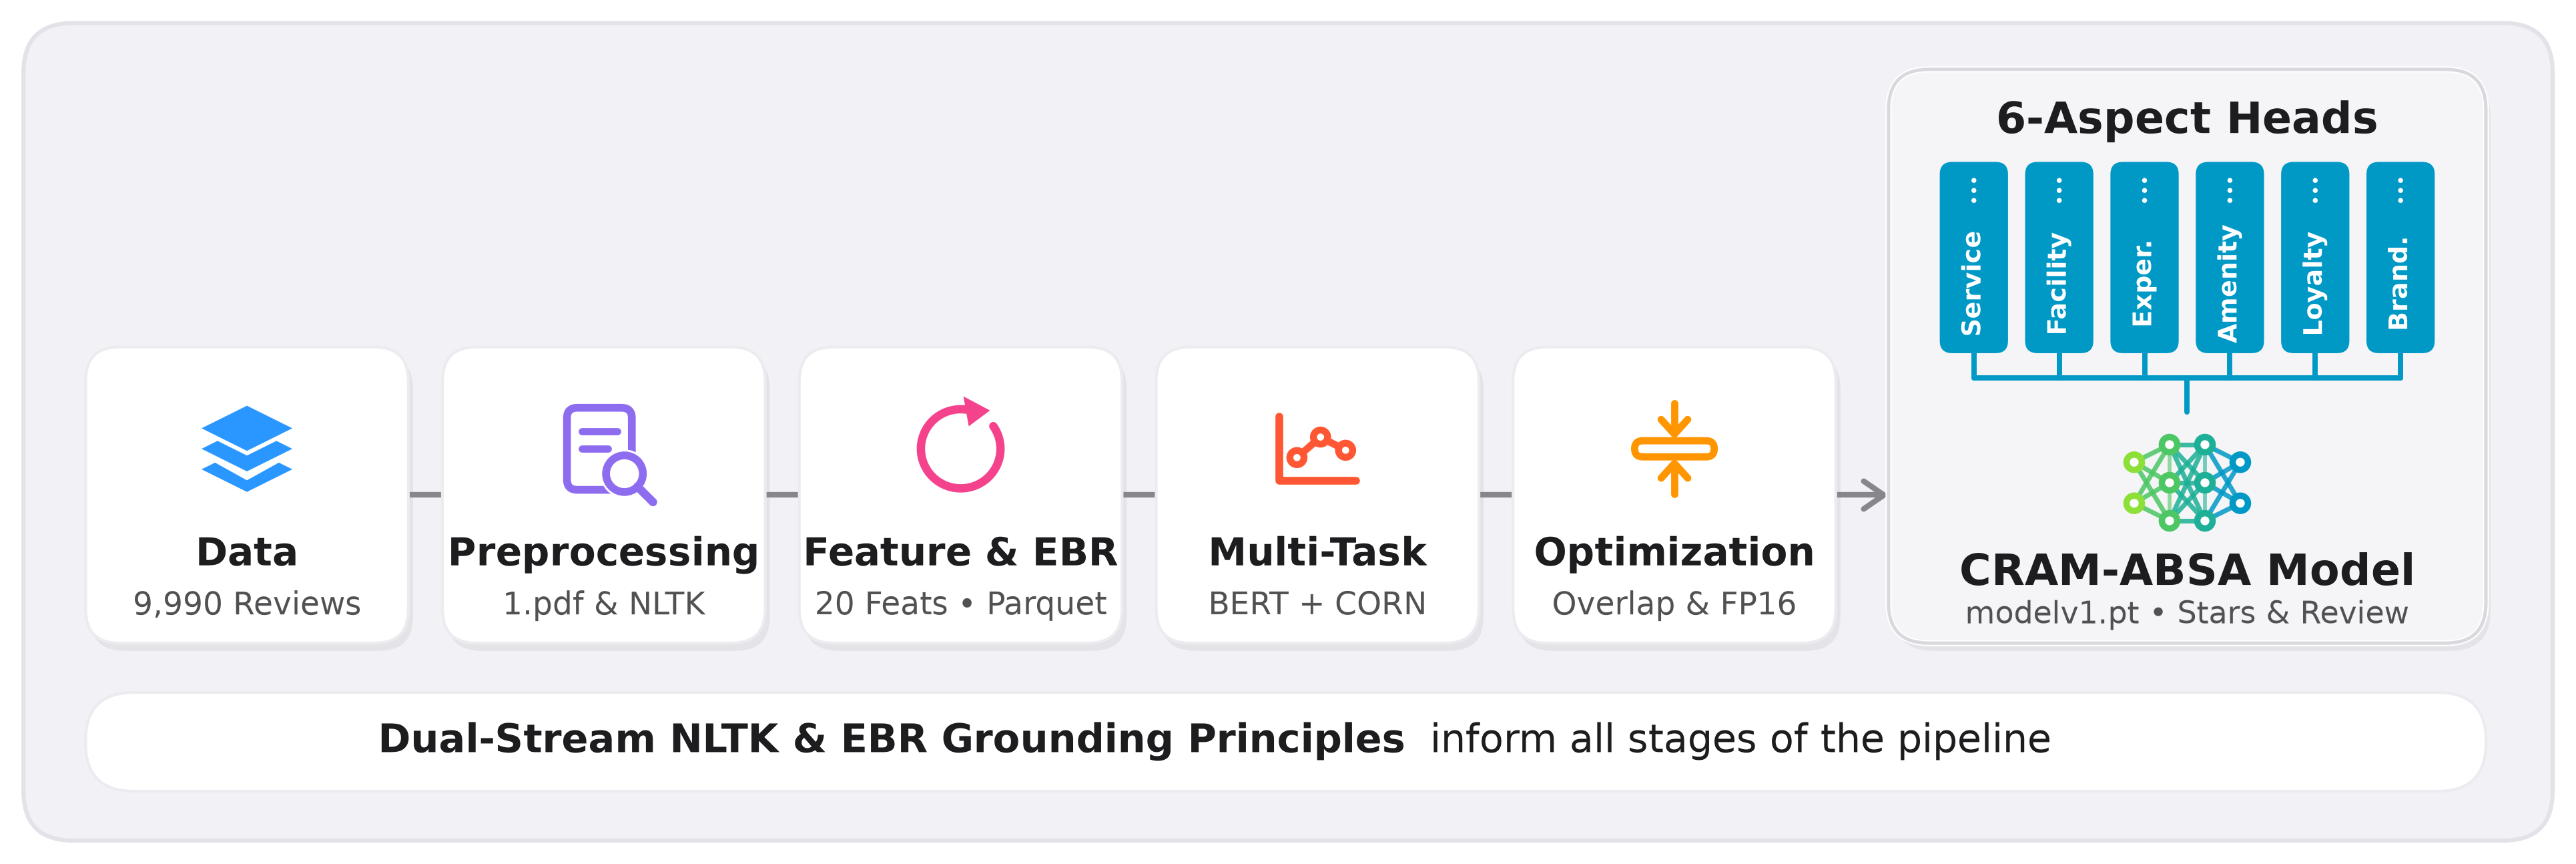
\includegraphics[width=1.22\textwidth]{chart_img/411_research_pipeline.png}}
    \caption{Sơ đồ quy trình nghiên cứu (Research Pipeline) của khung kiến trúc CRAM-ABSA qua 5 giai đoạn.}
    \label{fig:research_pipeline}
\end{figure}


Chi tiết 5 giai đoạn của quy trình nghiên cứu:
\begin{enumerate}
    \item \textbf{Giai đoạn 01 -- Thu thập Dữ liệu \& Gán nhãn Đa khía cạnh (Data Ingestion \& Span Annotation):} Khai thác tập dữ liệu gồm 9,990 bài đánh giá khách sạn tiếng Anh từ TripAdvisor (\texttt{TripAdvisor\_EN.json}) trên toàn lãnh thổ Việt Nam. Toàn bộ các bài đánh giá được dán nhãn mức đoạn văn (span-level) tạo thành 54,326 chú thích căn cứ (rationales) bao phủ 6 khía cạnh chuẩn cốt lõi: \textit{Service} (thái độ lễ tân, buồng phòng), \textit{Facility} (phòng ốc, vệ sinh, cách âm), \textit{Experience} (cảm nhận, trải nghiệm lưu trú), \textit{Amenity} (bể bơi, spa, gym, buffet, wifi), \textit{Loyalty} (mức độ trung thành, ý định quay lại) và \textit{Branding} (danh tiếng, đẳng cấp thương hiệu). Mỗi đoạn trích dẫn được liên kết trực tiếp với nhãn cảm xúc tương ứng (\textit{Positive, Neutral, Negative}) cùng siêu dữ liệu đầy đủ (hạng sao, điểm đánh giá 1--5 sao, ngày tháng đăng bài).
    
    \item \textbf{Giai đoạn 02 -- Tiền xử lý Dữ liệu Hai Luồng (Dual-Stream NLTK Cleaning) \& Kiểm định Rò rỉ Ngữ nghĩa (Cross-Aspect Leakage EDA):} Thực hiện chuẩn hóa văn bản theo chuẩn Unicode NFC trên luồng chính để bảo toàn tuyệt đối tọa độ ký tự \texttt{start\_char}/\texttt{end\_char} cho BERT, đồng thời áp dụng luồng xử lý ngôn ngữ tự nhiên NLTK có bảo toàn phủ định (kế thừa cải tiến từ~\cite{bimaputra2023aspect}) trên luồng phụ để trích xuất đặc trưng từ vựng. Khám phá phân vị độ dài (trung bình 350.7 ký tự, 82.1 từ) xác nhận phạm vi độ dài hoàn toàn tương thích với giới hạn chuỗi đầu vào của BERT. Thiết lập ma trận đồng xuất hiện giữa các khía cạnh và định lượng mức độ chồng lấn tọa độ span (\textit{Cross-Aspect Span Overlap}) làm cơ sở thực nghiệm trả lời \textbf{RQ2}, đồng thời phân tích độ lệch dữ liệu cực đoan (71.55\% điểm 5 sao) đặt nền móng cho \textbf{RQ1}.
    
    \item \textbf{Giai đoạn 03 -- Kỹ thuật 20 Đặc trưng \& Hạ tầng Tri thức Parquet/SQLite (20-Feature Engineering \& EBR Store):} Xây dựng cơ sở dữ liệu SQLite (\texttt{chatbot.db}) và xuất bản tệp Apache Parquet nén Snappy (\texttt{hotel\_reviews.parquet}, gồm 9,990 dòng và 44 cột sau phân tầng) hỗ trợ nạp dữ liệu tốc độ cao vào GPU. Trích xuất **20 đặc trưng định lượng** bao phủ 6 khía cạnh: 17 đặc trưng cấu trúc, mật độ bằng chứng, điểm cảm xúc liên tục trên 6 khía cạnh, cờ xung đột, suy giảm thời gian ($\lambda = 0.03$) đã được điều chỉnh để hoạt động cả khi nhận review mới, kết hợp cùng **3 đặc trưng NLP/NLTK \& EBR mới** (\texttt{feat\_nltk\_clean\_token\_ratio}, \texttt{feat\_nltk\_opinion\_negation\_density}, \texttt{feat\_ebr\_aspect\_prototype\_sim}).
    
    \item \textbf{Giai đoạn 04 -- Huấn luyện Mô hình CRAM-ABSA (BERT Backbone) Đa GPU trên Kaggle T4x2 (\texttt{trainv1.ipynb}):} Khởi tạo mô hình \texttt{bert-base-uncased} tích hợp trong kiến trúc CRAM-ABSA, tối ưu hóa cho cụm phần cứng **Kaggle Dual GPU T4x2 (30GB VRAM)** thông qua cơ chế song song dữ liệu (\texttt{nn.DataParallel}) và Mixed Precision FP16 (\texttt{torch.amp.autocast}). Kết hợp module truy xuất dựa trên nhúng (\textit{Embedding-Based Retrieval -- EBR}), mạng chiếu phi tuyến (\textit{Dense Feature Projection}) dung hợp vector 20 đặc trưng, và bộ tạo mặt nạ căn cứ mềm $m_a \in [0, 1]^L$. Tối ưu hóa đồng thời hàm mất mát đa nhiệm gồm mất mát sinh nhận xét 6 khía cạnh, mất mát thứ bậc CORN (\textbf{RQ1, RQ2}) và hình phạt chồng lấn phân đoạn $\mathcal{L}_{\text{overlap}}$ (\textbf{RQ2, RQ3}).
    
    \item \textbf{Giai đoạn 05 -- Đánh giá Thực nghiệm Toàn diện \& Sinh Nhận xét cho Review Mới (\texttt{benchmark.ipynb}):} Thực thi đánh giá hậu huấn luyện trên tập kiểm thử độc lập (999 bài đánh giá) nhằm kiểm chứng định lượng ba câu hỏi nghiên cứu (\textbf{RQ1, RQ2, RQ3}) qua các chỉ số \textbf{Acc@0}, \textbf{6-Aspect Macro-F1}, \textbf{Macro-MAE}, \textbf{Rationale Token-F1 / Leakage Rate}, \textbf{Commentary Token-F1} và \textbf{ROUGE-L}, đồng thời kiểm thử trực tiếp khả năng sinh bảng đánh giá và lời nhận xét chi tiết trên 6 khía cạnh khi đưa vào các bài đánh giá khách sạn mới.
\end{enumerate}

\subsection{Dữ liệu \& Thu thập - Data Collecting}
\label{subsec:datacollecting}

Nghiên cứu này sử dụng bộ dữ liệu đánh giá khách sạn bằng tiếng Anh từ TripAdvisor, lưu trong tệp \texttt{TripAdvisor\_EN.json}, bao gồm 9,990 bài đánh giá với tổng cộng 54,326 chú thích ở cấp độ đoạn văn bản. Mỗi bài đánh giá thể hiện trải nghiệm thực tế của khách hàng về khách sạn tại Việt Nam và được gán nhãn phù hợp với các khía cạnh và cảm xúc tương ứng.

Cấu trúc tệp JSON gồm ba thành phần chính: 
1. \textbf{data.text:} Chứa nội dung nguyên bản của bài đánh giá.
2. \textbf{meta\_info:} Cung cấp thông tin bổ sung như mã tham chiếu, tên khách sạn, địa điểm, điểm đánh giá và thời gian.
3. \textbf{annotations:} Lưu trữ kết quả gán nhãn. Mỗi chú thích xác định đoạn văn bản bằng chứng thông qua tọa độ bắt đầu (\texttt{start}) và kết thúc (\texttt{end}), đồng thời liên kết đoạn văn bản với khía cạnh và nhãn cảm xúc tương ứng.

Bộ dữ liệu được phân chia thành sáu khía cạnh chuẩn: 
- \textbf{Service} (dịch vụ, thái độ phục vụ của nhân viên)
- \textbf{Facility} (cơ sở vật chất, phòng nghỉ, vệ sinh, cách âm)
- \textbf{Experience} (trải nghiệm lưu trú tổng thể, cảm nhận kỳ nghỉ)
- \textbf{Amenity} (tiện ích đi kèm: hồ bơi, ẩm thực bữa sáng, spa, gym, wifi)
- \textbf{Loyalty} (lòng trung thành, ý định quay lại hoặc giới thiệu)
- \textbf{Branding} (thương hiệu, danh tiếng, mức độ tương xứng hạng sao)

Nhãn được gán ở cấp độ đoạn văn bản thay vì áp dụng một nhãn chung cho toàn bộ bài đánh giá, cho phép một bài đánh giá có thể chứa nhiều đoạn bằng chứng thuộc các khía cạnh khác nhau và các sắc thái cảm xúc khác nhau. Cấu trúc này cung cấp nền tảng lý tưởng để huấn luyện mô hình CRAM-ABSA học cách định vị bằng chứng và sinh nhận xét độc lập cho từng khía cạnh trong số 6 khía cạnh khi tiếp nhận một bài đánh giá mới.


\subsection{Tiền xử lý \- Data Preprocessing (EDA) \& Kỹ thuật 20 Đặc trưng}
\label{subsec:datapreprocessing}

Quy trình tiền xử lý dữ liệu và kỹ thuật đặc trưng trong \texttt{Project.ipynb} được thực hiện bằng Python với các thư viện \textbf{\texttt{orjson}, \texttt{pandas}, \texttt{nltk}, SQLite và PyArrow} theo các bước chi tiết như sau:

A. Đọc dữ liệu và Tiền xử lý Ngôn ngữ Tự nhiên Hai Luồng (Dual-Stream NLP/NLTK Flow).

Tệp JSON chứa 9,990 bản ghi được đọc bằng \textbf{\texttt{orjson}} và xử lý theo kiến trúc hai luồng song song nhằm kế thừa ưu điểm làm sạch văn bản của Bimaputra \& Sutoyo~\cite{bimaputra2023aspect} mà không phá vỡ cấu trúc ngữ cảnh của BERT và CRAM-ABSA:
- \textbf{Luồng 1 -- Chuẩn hóa bảo toàn tọa độ cho BERT Backbone \& Span Alignment:} Văn bản gốc được chuẩn hóa theo định dạng Unicode NFC và loại bỏ khoảng trắng thừa ở hai đầu nhưng giữ nguyên dấu câu, từ dừng và độ dài ký tự nhằm bảo toàn chính xác tuyệt đối các tọa độ \texttt{start\_char}/\texttt{end\_char} của 54,326 đoạn bằng chứng.
- \textbf{Luồng 2 -- Làm sạch văn bản bằng NLTK có bảo toàn phủ định (Negation-Aware NLTK Cleaning):} Văn bản được chuyển về chữ thường, mở rộng các cấu trúc viết tắt tiếng Anh (\textit{don't $\to$ do not, couldn't $\to$ could not, won't $\to$ will not}), loại bỏ thẻ nhiễu/ký tự đặc biệt và lọc từ dừng bằng thư viện \textbf{NLTK} nhưng \textbf{giữ lại toàn bộ nhóm từ phủ định và chuyển ý} (\textit{not, no, never, neither, without, but, however, although, fault}). Thiết kế này khắc phục triệt để nhược điểm làm mất từ \textit{not} khi xóa stopwords thông thường, đồng thời cung cấp chuỗi từ khóa sạch cho tầng truy xuất EBR và trích xuất 3 đặc trưng ngôn ngữ học mới.

B. Chuyển dữ liệu thành hai bảng quan hệ.

Dữ liệu từ JSON được tách ra thành hai bảng liên kết qua \texttt{review\_id}:
- \textbf{\texttt{reviews}:} Bao gồm 16 cột chứa thông tin khách sạn, điểm đánh giá, thời gian, nội dung review, độ dài và các nhãn dẫn xuất.
- \textbf{\texttt{aspect\_annotations}:} Lưu trữ 54,326 đoạn bằng chứng với thông tin về khía cạnh, cảm xúc, tọa độ và nội dung trích đoạn.

C. Kiểm tra chất lượng dữ liệu.

Quá trình kiểm định cho thấy cả hai bảng đều đạt 100\% độ hoàn thiện (0\% giá trị khuyết thiếu hoặc tọa độ không hợp lệ). Toàn bộ 9,990 bài đánh giá (nằm trong khoảng 30--150 từ) và 54,326 chú thích được bảo toàn nguyên vẹn.

D. Xây dựng và Mở rộng Hệ thống 20 Đặc trưng Định lượng (20-Feature Engineering).

Để phục vụ mục tiêu sinh đánh giá và nhận xét trên 6 khía cạnh khi đưa vào một bài review mới, hệ thống điều chỉnh 17 đặc trưng hiện hữu sang chế độ hoạt động kép (kết hợp span chú thích trong tập huấn luyện và bộ suy luận từ vựng NLTK khi nhận review mới) đồng thời bổ sung \textbf{3 đặc trưng mới} để hoàn thiện vector \textbf{20 đặc trưng} ($\mathbf{f} \in \mathbb{R}^{20}$):
- \textbf{Nhóm 1 -- Cấu trúc và mật độ bằng chứng (Features 1--2, 5--7, 14):} Số lượng khía cạnh xuất hiện (\texttt{feat\_aspect\_count}), mã số hóa khía cạnh chủ đạo (\texttt{feat\_dominant\_aspect} $\in \{0..6\}$), mật độ bằng chứng (\texttt{feat\_evidence\_density}), độ dài trung bình đoạn căn cứ (\texttt{feat\_avg\_rationale\_len}), cờ chồng lấn ranh giới liên khía cạnh (\texttt{feat\_has\_cross\_overlap}) và tỷ lệ bao phủ trên 6 khía cạnh chuẩn (\texttt{feat\_aspect\_coverage\_ratio}).
- \textbf{Nhóm 2 -- Cảm xúc tổng thể, xung đột và thời gian (Features 3--4, 15--17):} Điểm cảm xúc ròng (\texttt{feat\_net\_sentiment\_score}), cờ xung đột cảm xúc đa khía cạnh (\texttt{feat\_sentiment\_conflict}), trọng số suy giảm thời gian (\texttt{feat\_recency\_weight} với $\lambda = 0.03$), độ đồng thuận nội tại (\texttt{feat\_consensus\_strength}) và điểm cảm xúc khía cạnh theo chuỗi thời gian (\texttt{feat\_temporal\_aspect\_sentiment}).
- \textbf{Nhóm 3 -- Điểm phân cực liên tục trên 6 khía cạnh chuẩn (Features 8--13):} Sáu đặc trưng định lượng cảm xúc trên từng khía cạnh (\texttt{feat\_service\_sentiment}, \texttt{feat\_facility\_sentiment}, \texttt{feat\_experience\_sentiment}, \texttt{feat\_amenity\_sentiment}, \texttt{feat\_loyalty\_sentiment}, \texttt{feat\_branding\_sentiment}) nhận giá trị liên tục trong đoạn $[-1.0, +1.0]$ được tính theo trọng số độ dài đoạn căn cứ kết hợp bộ phân tích phủ định NLTK, phản ánh chính xác mức độ khen/chê trên từng khía cạnh.
- \textbf{Nhóm 4 -- Ba đặc trưng NLP/NLTK \& Truy xuất Nhúng EBR mới (Features 18--20):}
  \begin{enumerate}
      \item \texttt{feat\_nltk\_clean\_token\_ratio} (\textbf{Feature 18}): Tỷ lệ từ nội dung thực chất sau bước chuẩn hóa NLTK bảo toàn phủ định trên tổng số từ gốc (trung bình đạt $0.5464 \pm 0.0643$ trên toàn tập dữ liệu).
      \item \texttt{feat\_nltk\_opinion\_negation\_density} (\textbf{Feature 19}): Mật độ các từ biểu đạt quan điểm cảm xúc, trạng từ nhấn mạnh và cấu trúc phủ định/chuyển ý được nhận diện qua NLTK, giúp mô hình nắm bắt chính xác hiện tượng đảo cực cảm xúc.
      \item \texttt{feat\_ebr\_aspect\_prototype\_sim} (\textbf{Feature 20}): Điểm tương đồng Cosine trung bình giữa bài đánh giá và vector nguyên mẫu (Aspect Prototypes) của 6 khía cạnh trong không gian truy xuất EBR (trung bình đạt $0.3075 \pm 0.0975$), hỗ trợ truy xuất các mẫu nhận xét chuẩn xác nhất.
  \end{enumerate}

E. Phân tích khám phá dữ liệu (EDA):

Về độ dài văn bản, mỗi bài đánh giá có độ dài trung bình $350{,}7$ ký tự ($\approx 82{,}1$ từ), trung vị 398 ký tự ($\approx 72$ từ), dao động từ 177 đến 847 ký tự ($30$--$150$ từ). Khoảng dao động gọn gàng này hoàn toàn tương thích với giới hạn chuỗi đầu vào (maximum sequence length) của các mô hình Transformer mà không cần cắt tỉa gây mất mát ngữ cảnh. Điểm đánh giá trung bình đạt $4{,}52$ đến $5{,}00$ sao (độ lệch chuẩn khoảng $0{,}89$), thể hiện xu hướng đánh giá tích cực áp đảo trong tập dữ liệu (71.55\% là đánh giá 5 sao).


\begin{figure}[H]
    \centering
    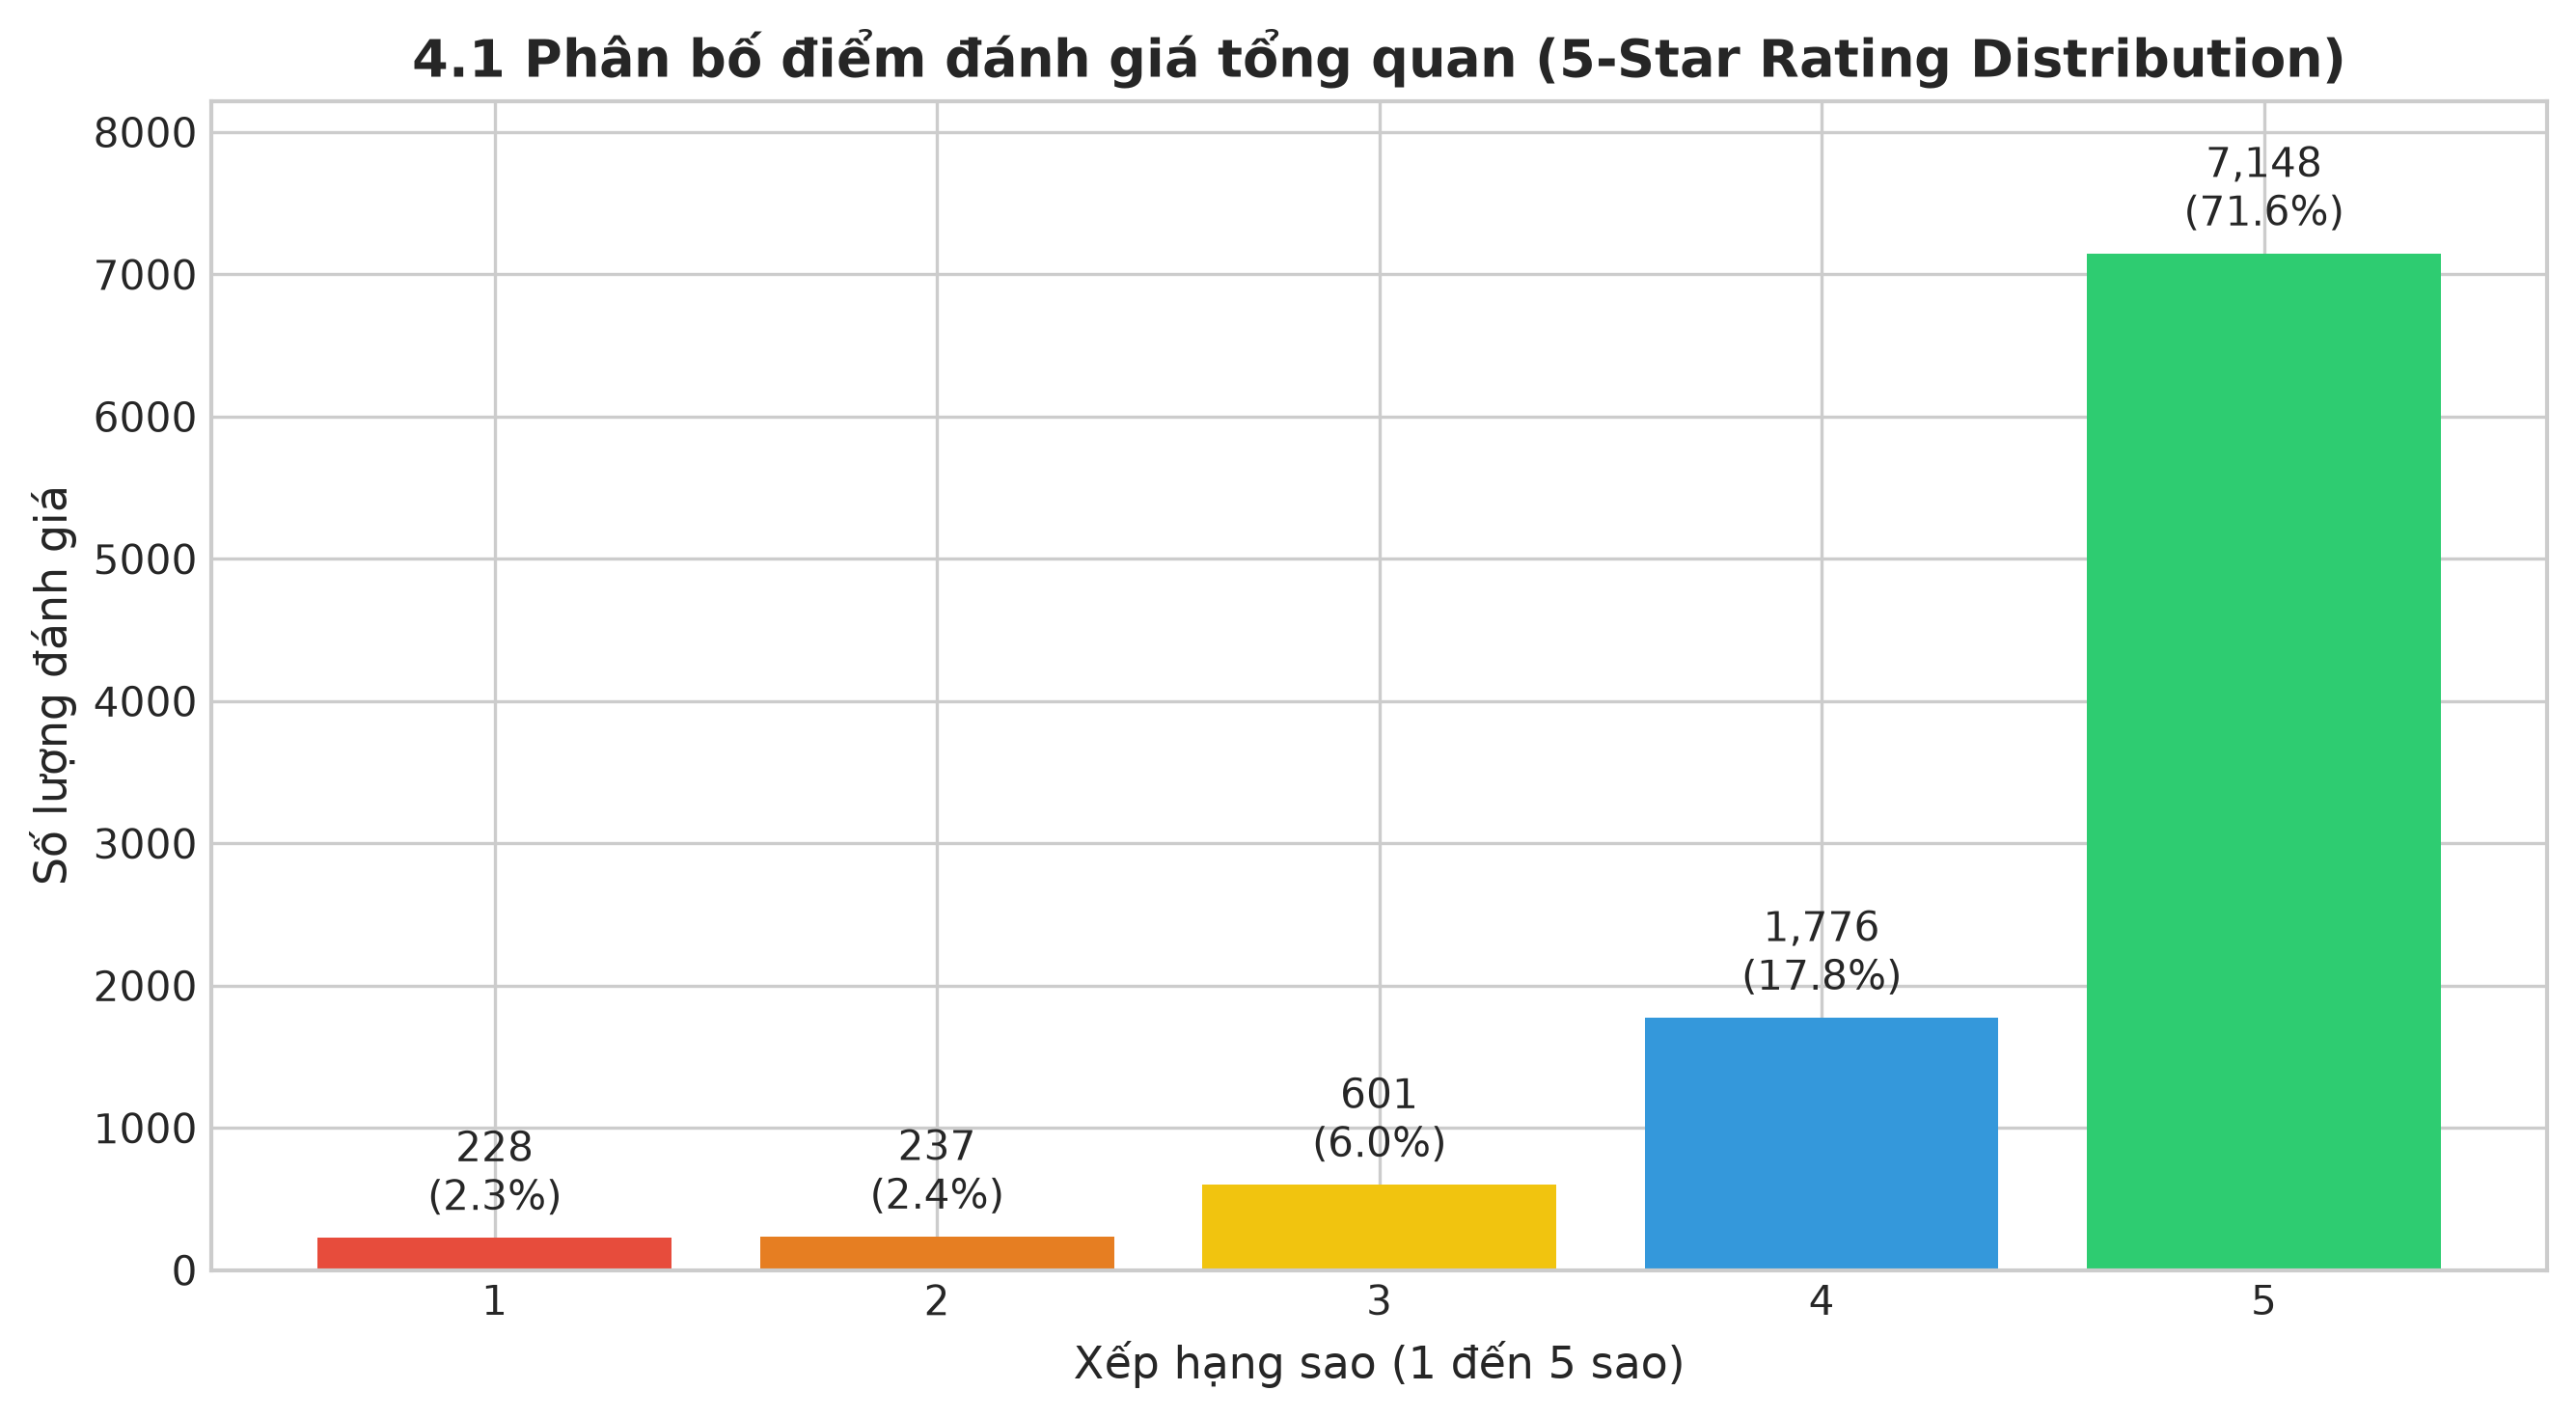
\includegraphics[width=0.8\linewidth]{chart_img/41_overall_rating_distribution.png}
    \caption{Phân bố điểm đánh giá.}
    \label{fig}
\end{figure}

Phân bố đánh giá phản ánh trải nghiệm thực tế của du khách tại các khách sạn ở các trung tâm du lịch lớn của Việt Nam (Hà Nội, TP. Hồ Chí Minh, Hội An). Khách sạn có số lượng đánh giá cao nhất (Sofitel Legend Metropole Hà Nội) sở hữu 85 bài (chiếm 0,9\% dữ liệu), và 10 khách sạn hàng đầu cộng lại chỉ chiếm khoảng 6,0\% (598 bài), cho thấy dữ liệu có độ phân tán tốt, không bị chi phối bởi một vài cơ sở lưu trú cục bộ (Hình~\ref{fig:top10_hotels}). Về tương quan độ dài, các bài đánh giá tiêu cực (1 sao) thường có xu hướng giải thích chi tiết hơn với độ dài trung bình khoảng 101 từ, dài hơn đáng kể so với các đánh giá tích cực 5 sao (trung bình khoảng 60 từ).

\begin{figure}[H]
    \centering
    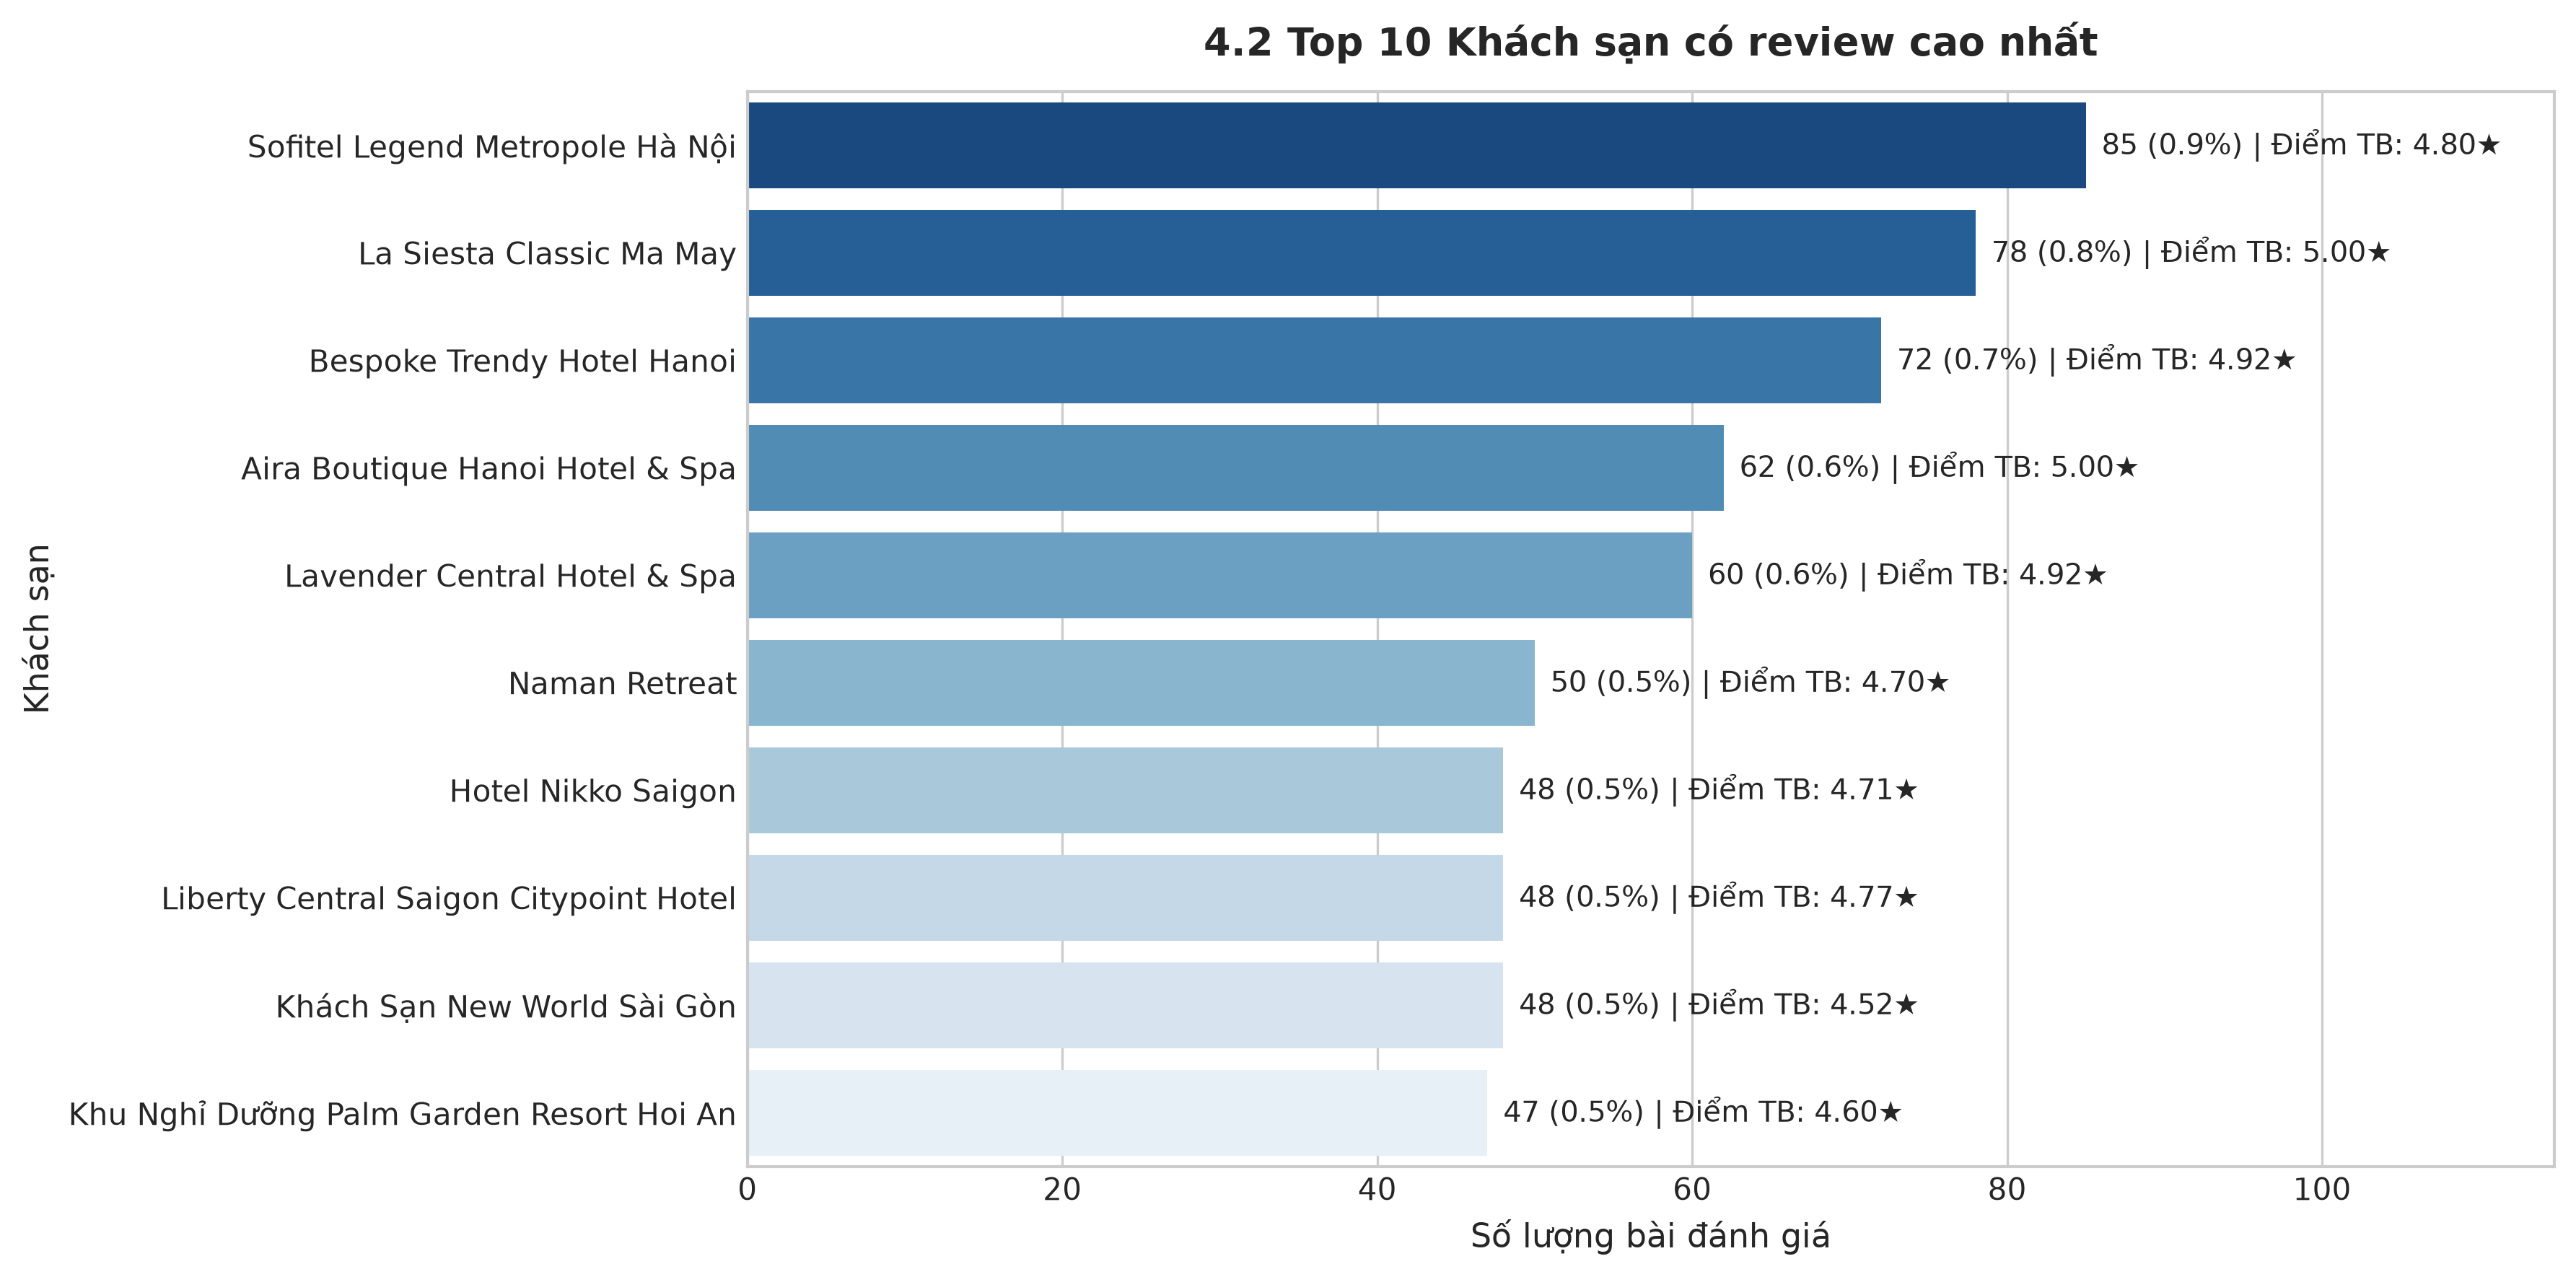
\includegraphics[width=0.8\linewidth]{chart_img/42_top10_hotels_highest_reviews.png}
    \caption{Top 10 khách sạn có nhiều bài đánh giá nhất trong tập dữ liệu.}
    \label{fig:top10_hotels}
\end{figure}

Tần suất xuất hiện của 6 khía cạnh chuẩn có sự phân hóa đáng kể (Hình~\ref{fig:aspect_freq_dist}). Trong đó, \textit{Service} chiếm tỷ trọng lớn nhất với 19.289 đoạn căn cứ (35,5\% tổng số chú thích, xuất hiện trong 91,4\% số bài đánh giá), tiếp theo là \textit{Facility} (12.641 đoạn; 23,3\%), \textit{Experience} (9.113 đoạn; 16,8\%) và \textit{Amenity} (7.651 đoạn; 14,1\%). Hai khía cạnh \textit{Loyalty} (4.293 đoạn; 7,9\%) và \textit{Branding} (1.339 đoạn; 2,5\%) chiếm tỷ lệ thấp hơn, phản ánh đặc thù hành vi khách hàng thường tập trung nhận xét về dịch vụ và phòng ốc trực tiếp.

\begin{figure}[H]
    \centering
    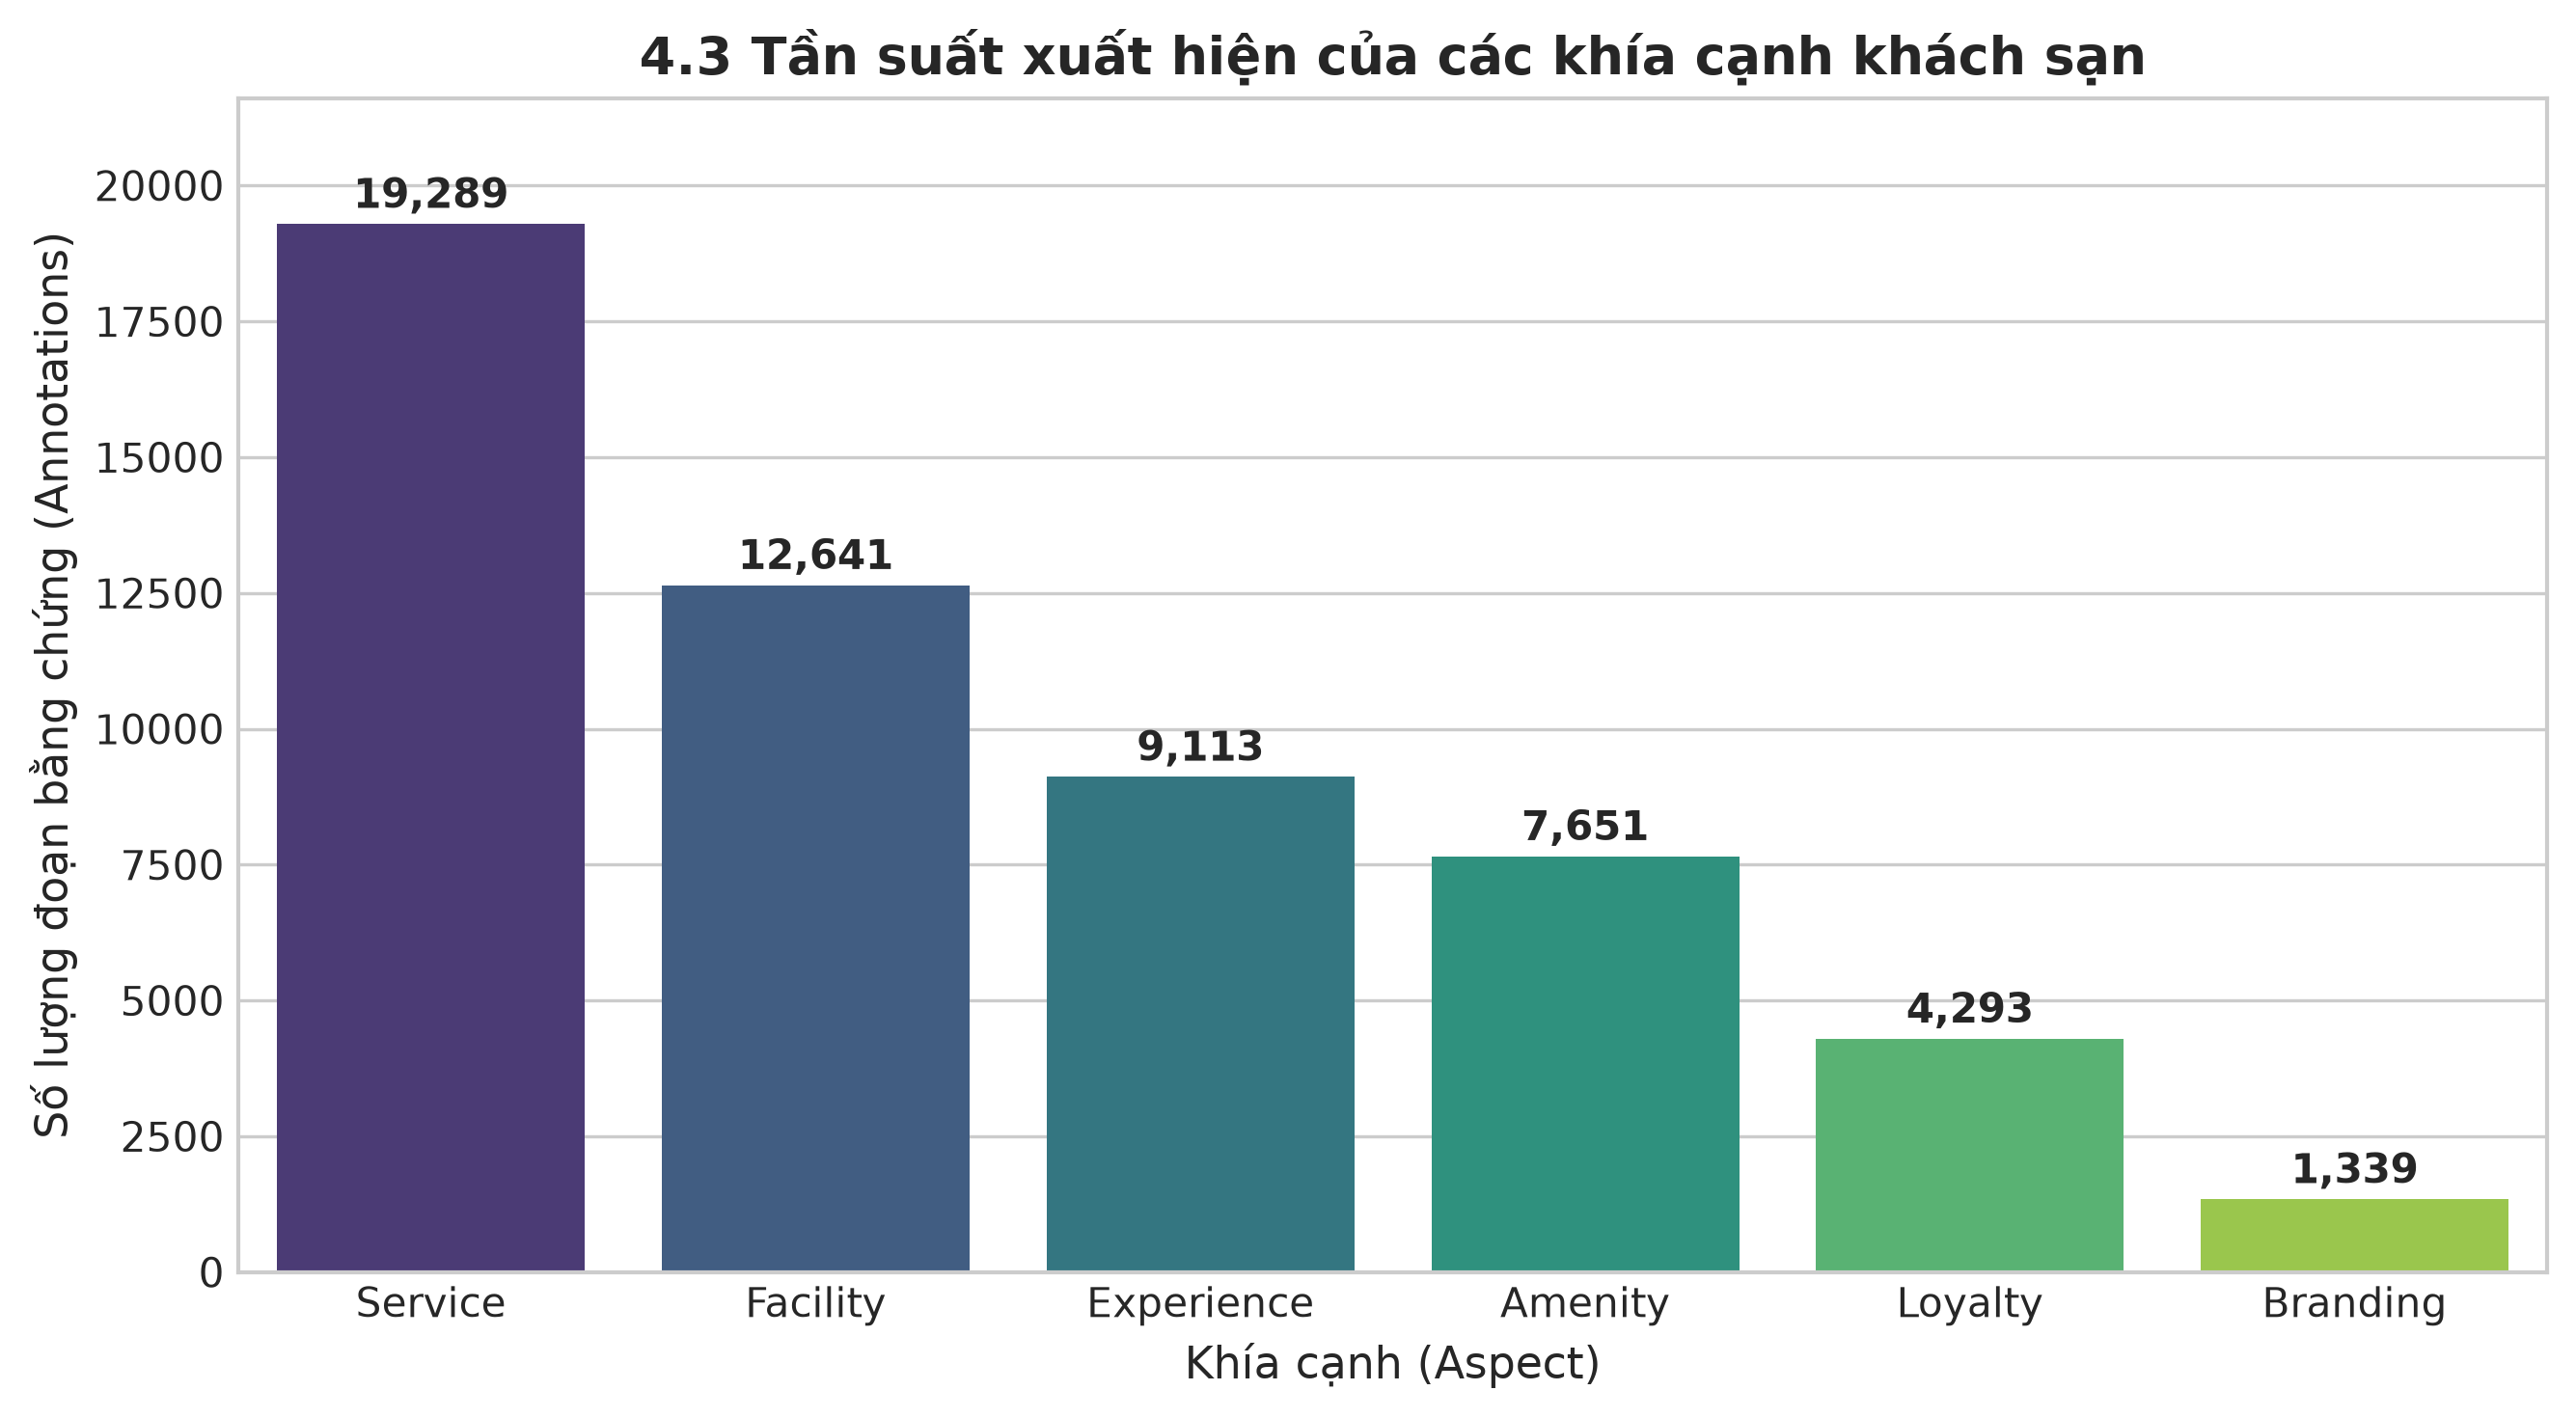
\includegraphics[width=0.8\linewidth]{chart_img/43_aspect_frequency_distribution.png}
    \caption{Tần suất xuất hiện của các khía cạnh.}
    \label{fig:aspect_freq_dist}
\end{figure}

Phân bố cảm xúc theo từng khía cạnh (Hình~\ref{fig:aspect_sent_breakdown}) cho thấy tỷ lệ tích cực chiếm ưu thế ở hầu hết các khía cạnh, cao nhất là \textit{Loyalty} (93,0\%), \textit{Service} (89,6\%) và \textit{Amenity} (89,0\%). Ngược lại, khía cạnh \textit{Facility} ghi nhận tỷ lệ tiêu cực cao nhất với 12,9\% (1.628 đoạn), cho thấy các phàn nàn của du khách chủ yếu phát sinh từ cơ sở vật chất phòng nghỉ.

\begin{figure}[H]
    \centering
    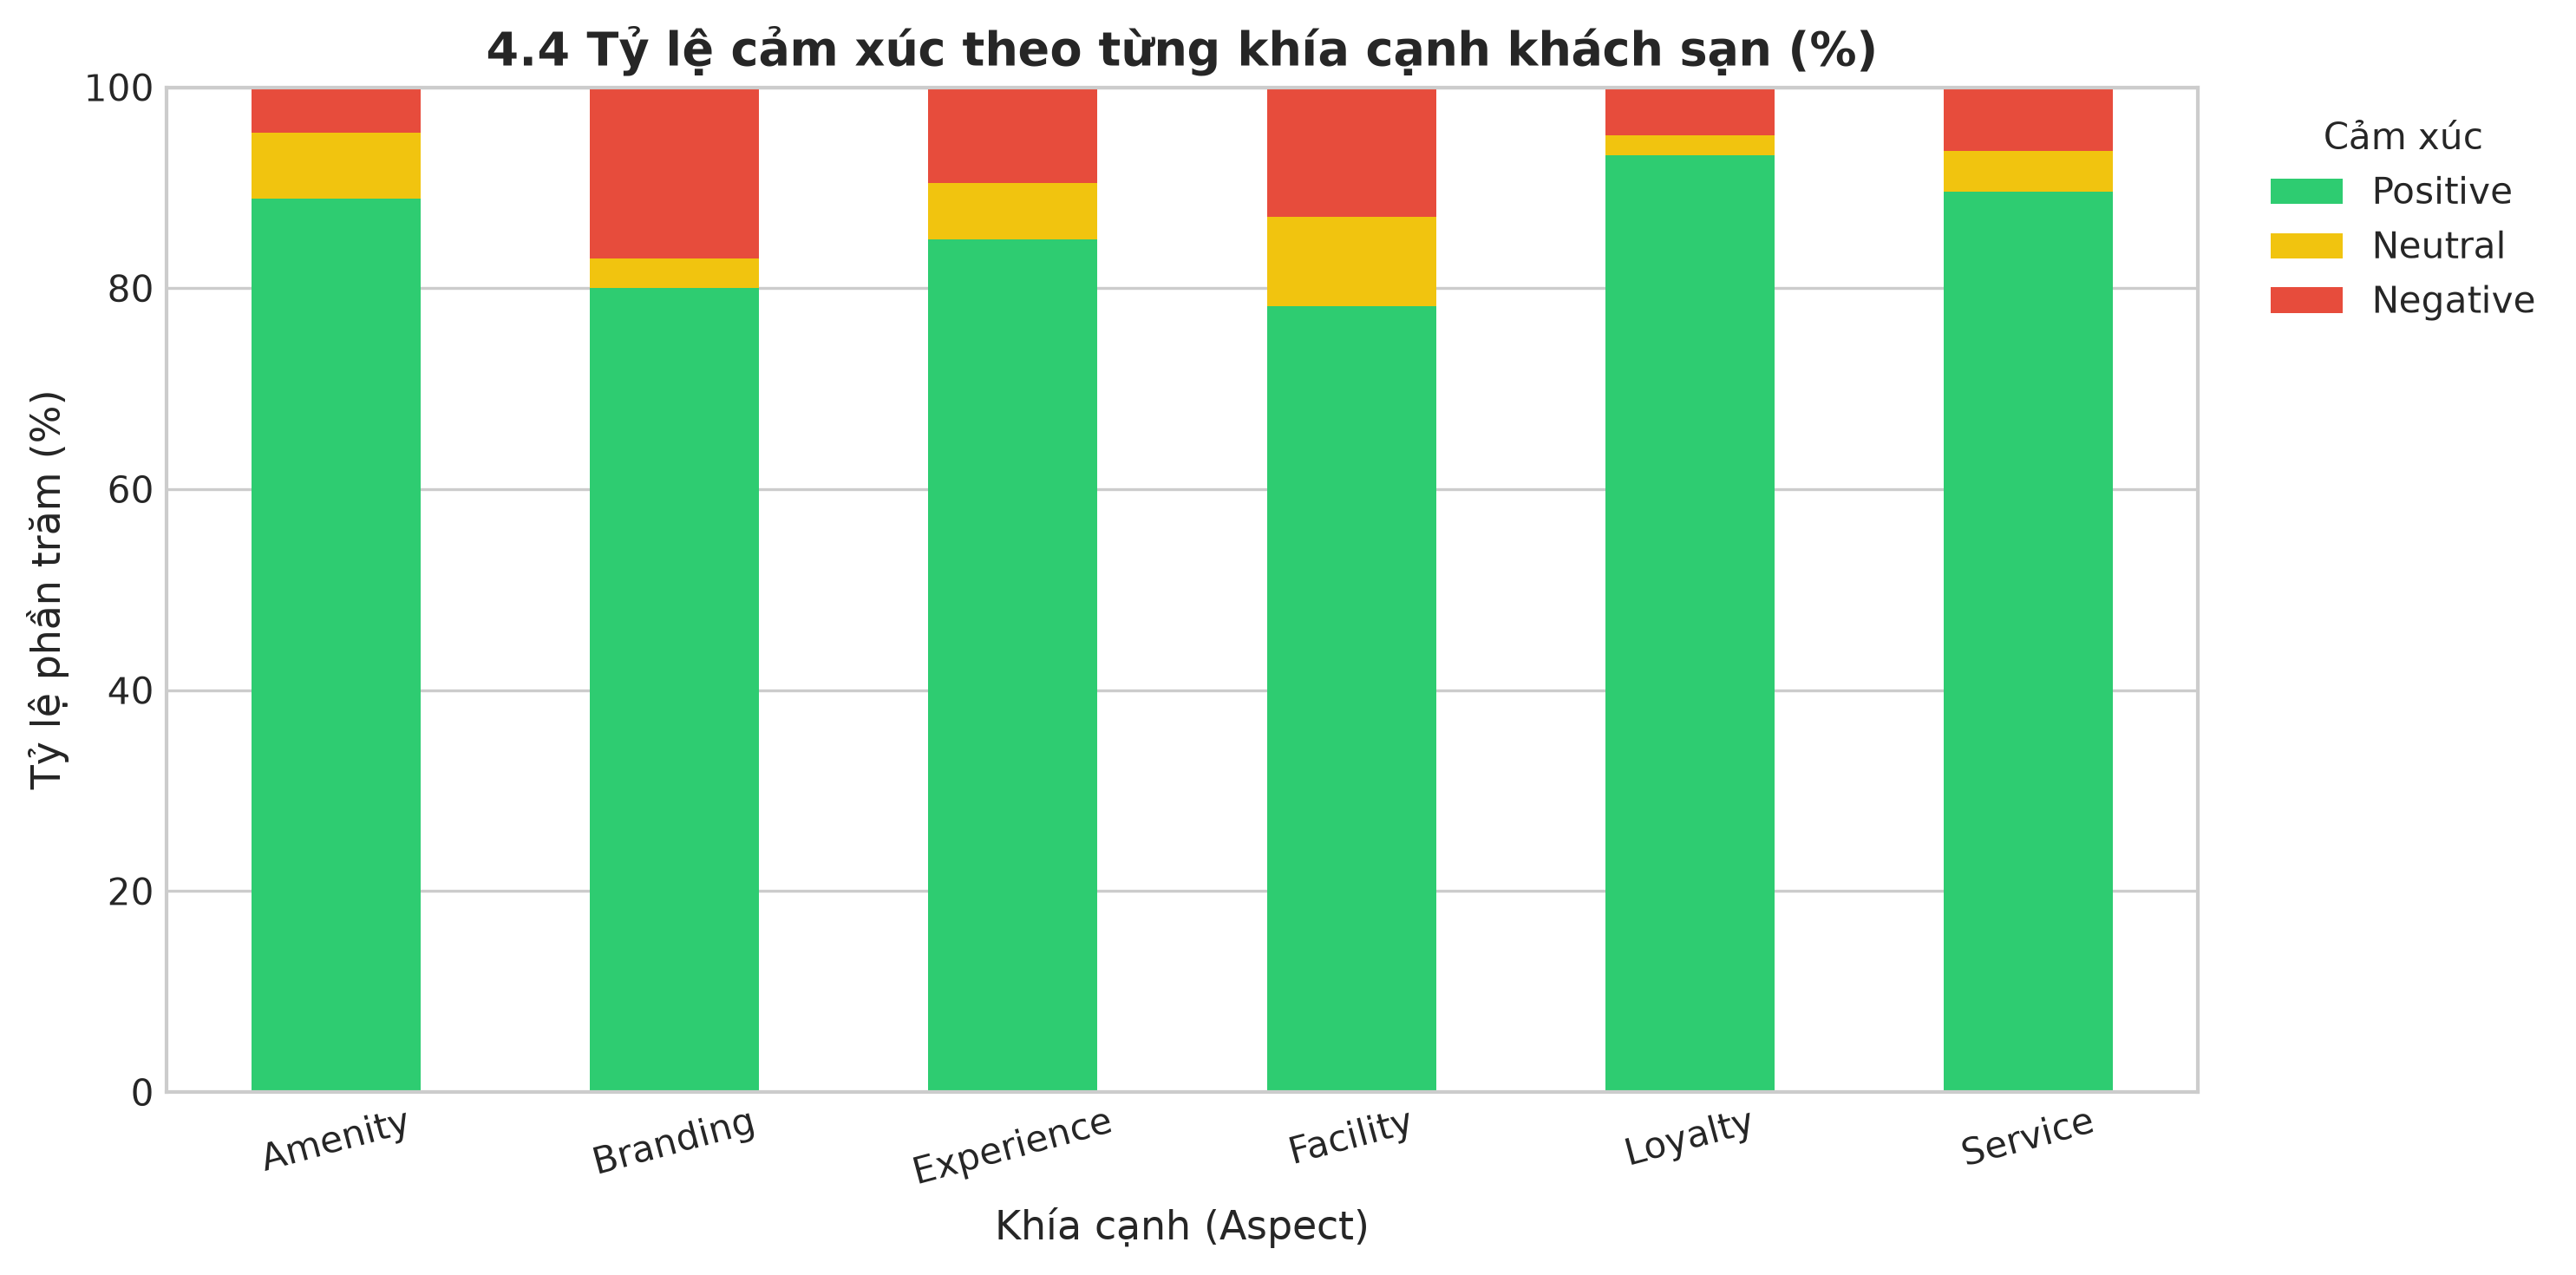
\includegraphics[width=0.75\linewidth]{chart_img/44_aspect_sentiment_breakdown.png}
    \caption{Tỷ lệ phân bố cảm xúc theo từng khía cạnh.}
    \label{fig:aspect_sent_breakdown}
\end{figure}

Về mức độ phức hợp của nội dung, hơn 68\% số bài đánh giá đề cập từ 3 đến 4 khía cạnh đồng thời (Hình~\ref{fig:aspects_per_review}), với trung bình 3,4 khía cạnh trên mỗi bài. Điều này đòi hỏi mô hình phải có khả năng phân rã đa nhãn chuẩn xác thay vì chỉ gán nhãn đơn cho toàn văn bản.

\begin{figure}[H]
    \centering
    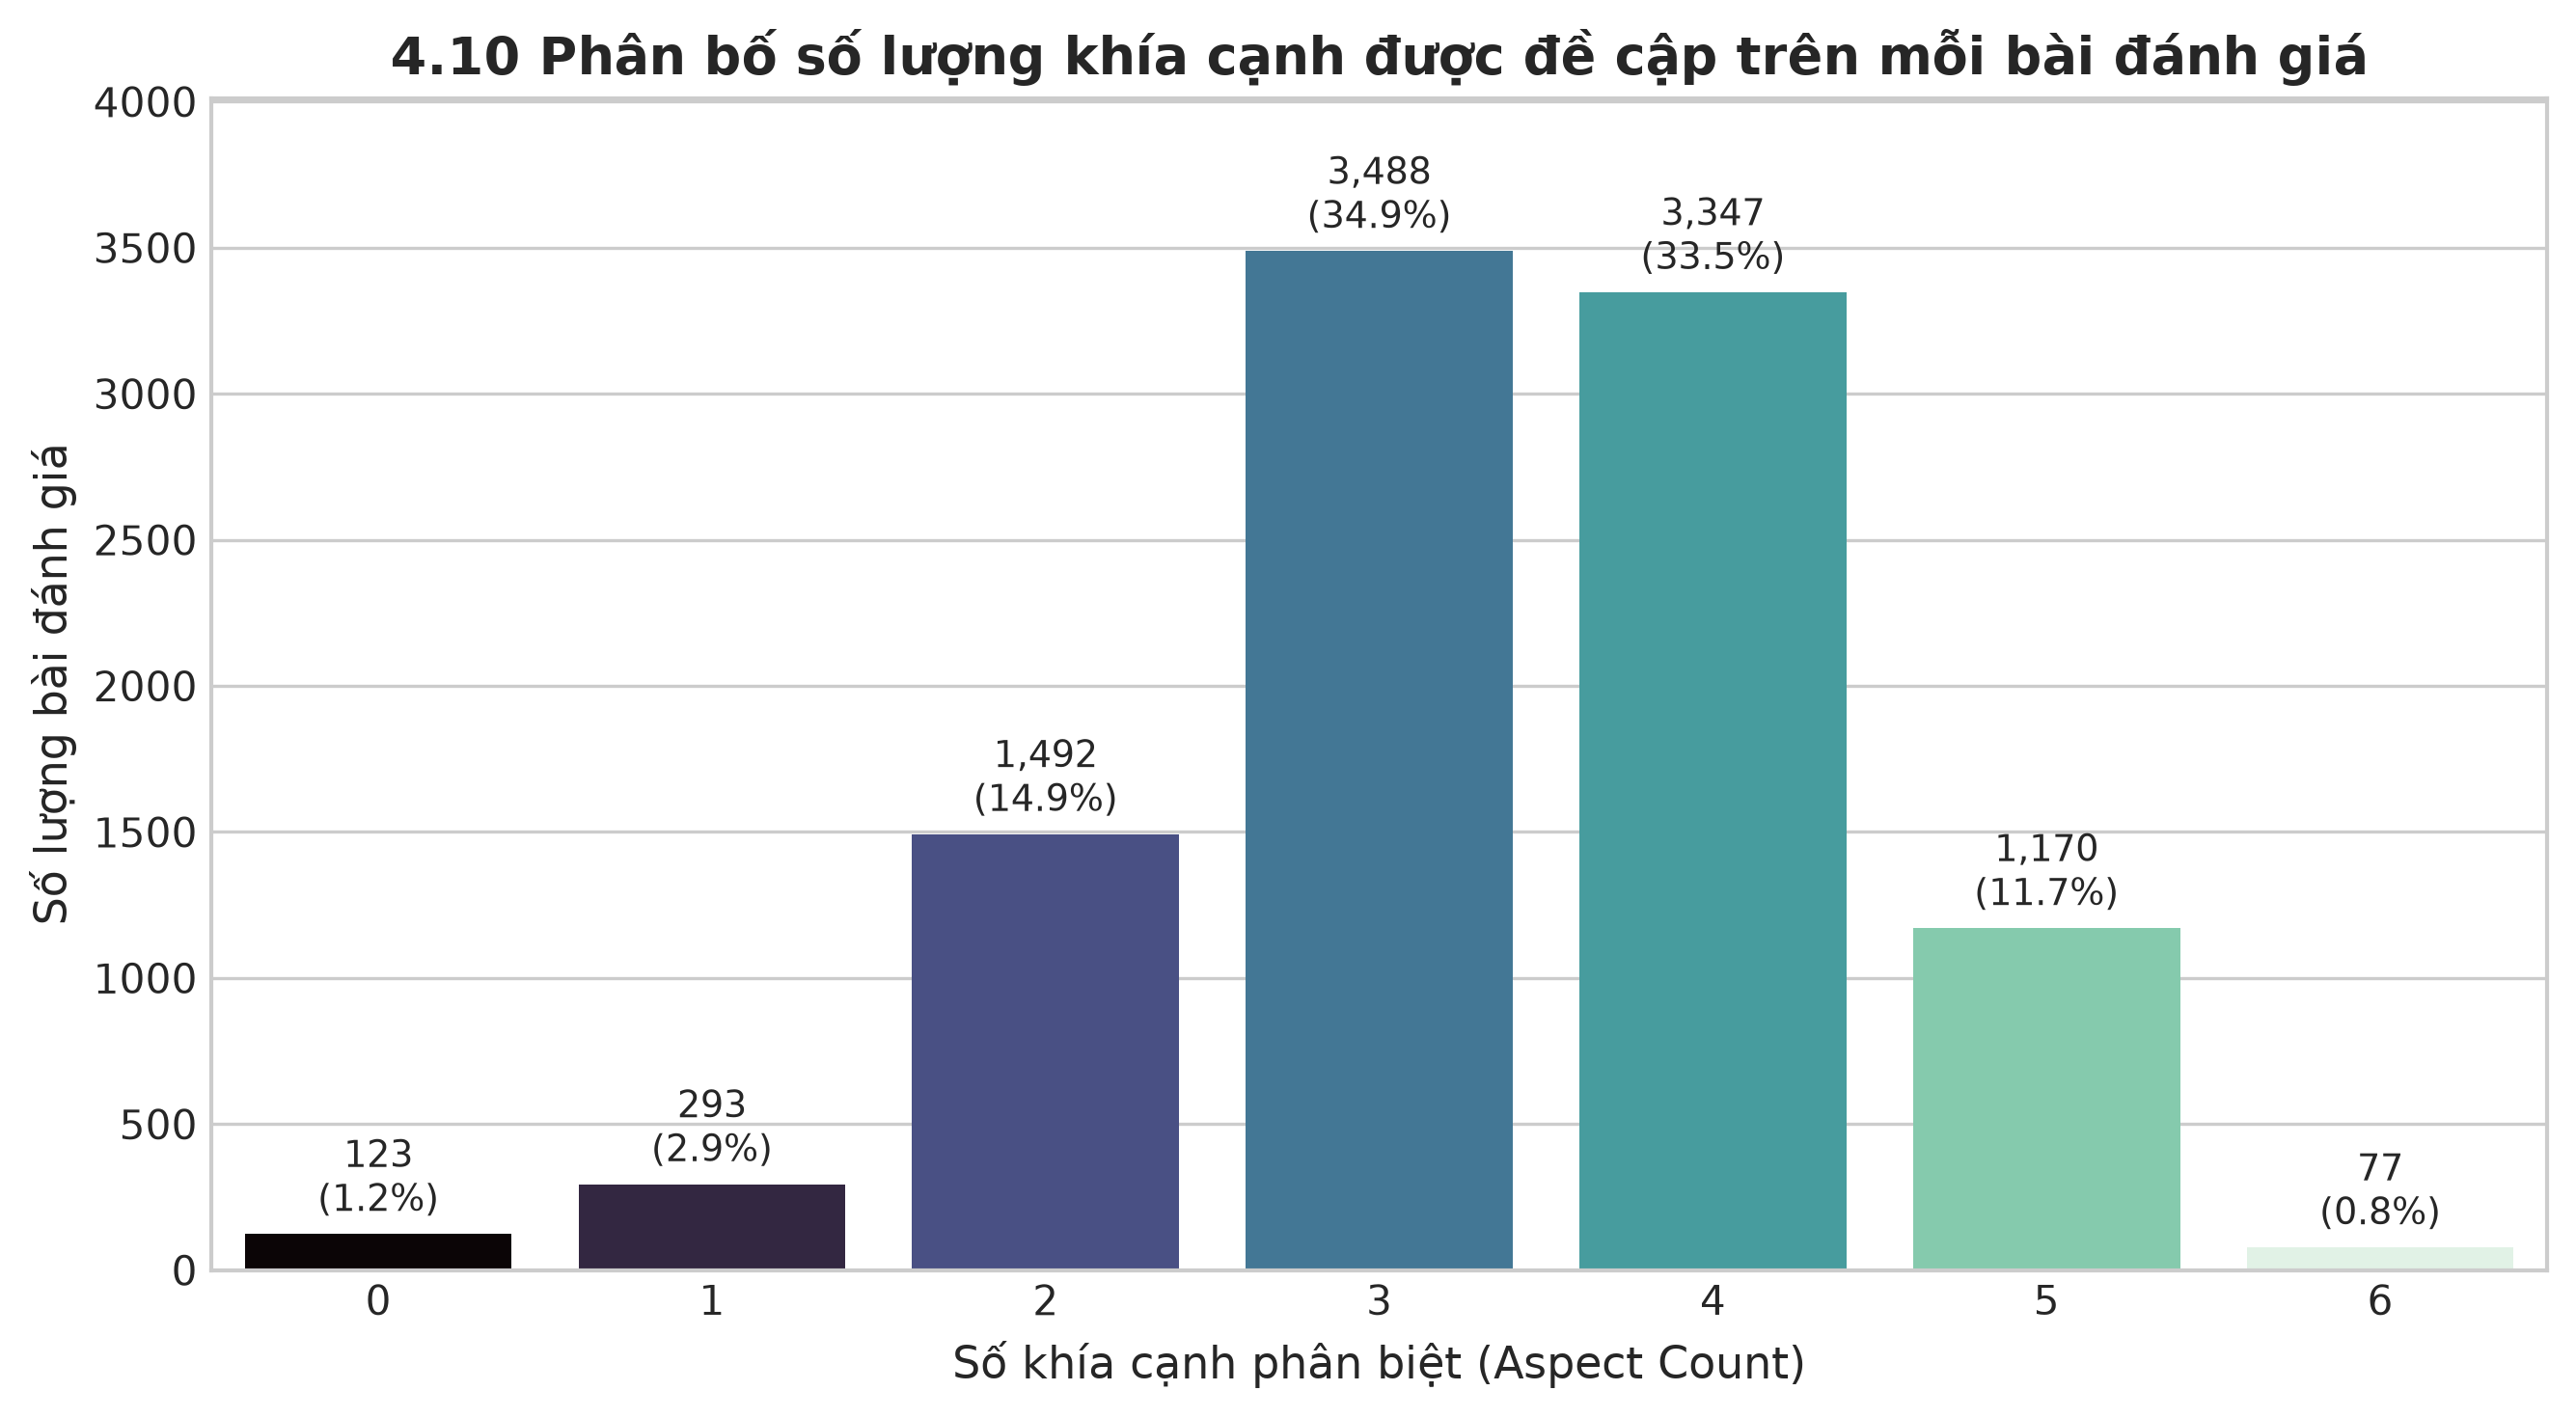
\includegraphics[width=0.75\linewidth]{chart_img/410_aspects_per_review_distribution.png}
    \caption{Phân bố số lượng khía cạnh được đề cập trong mỗi bài đánh giá.}
    \label{fig:aspects_per_review}
\end{figure}

Về đặc tính đoạn căn cứ (rationale spans), độ dài trung bình dao động từ 63 đến 74 ký tự (Hình~\ref{fig:rationale_len_aspect}), chiếm khoảng 14\% dung lượng văn bản của bài đánh giá. Các bài đánh giá 1 sao thường có đoạn căn cứ dài hơn so với đánh giá 5 sao do khách hàng có xu hướng miêu tả chi tiết các sự cố phát sinh.

\begin{figure}[H]
    \centering
    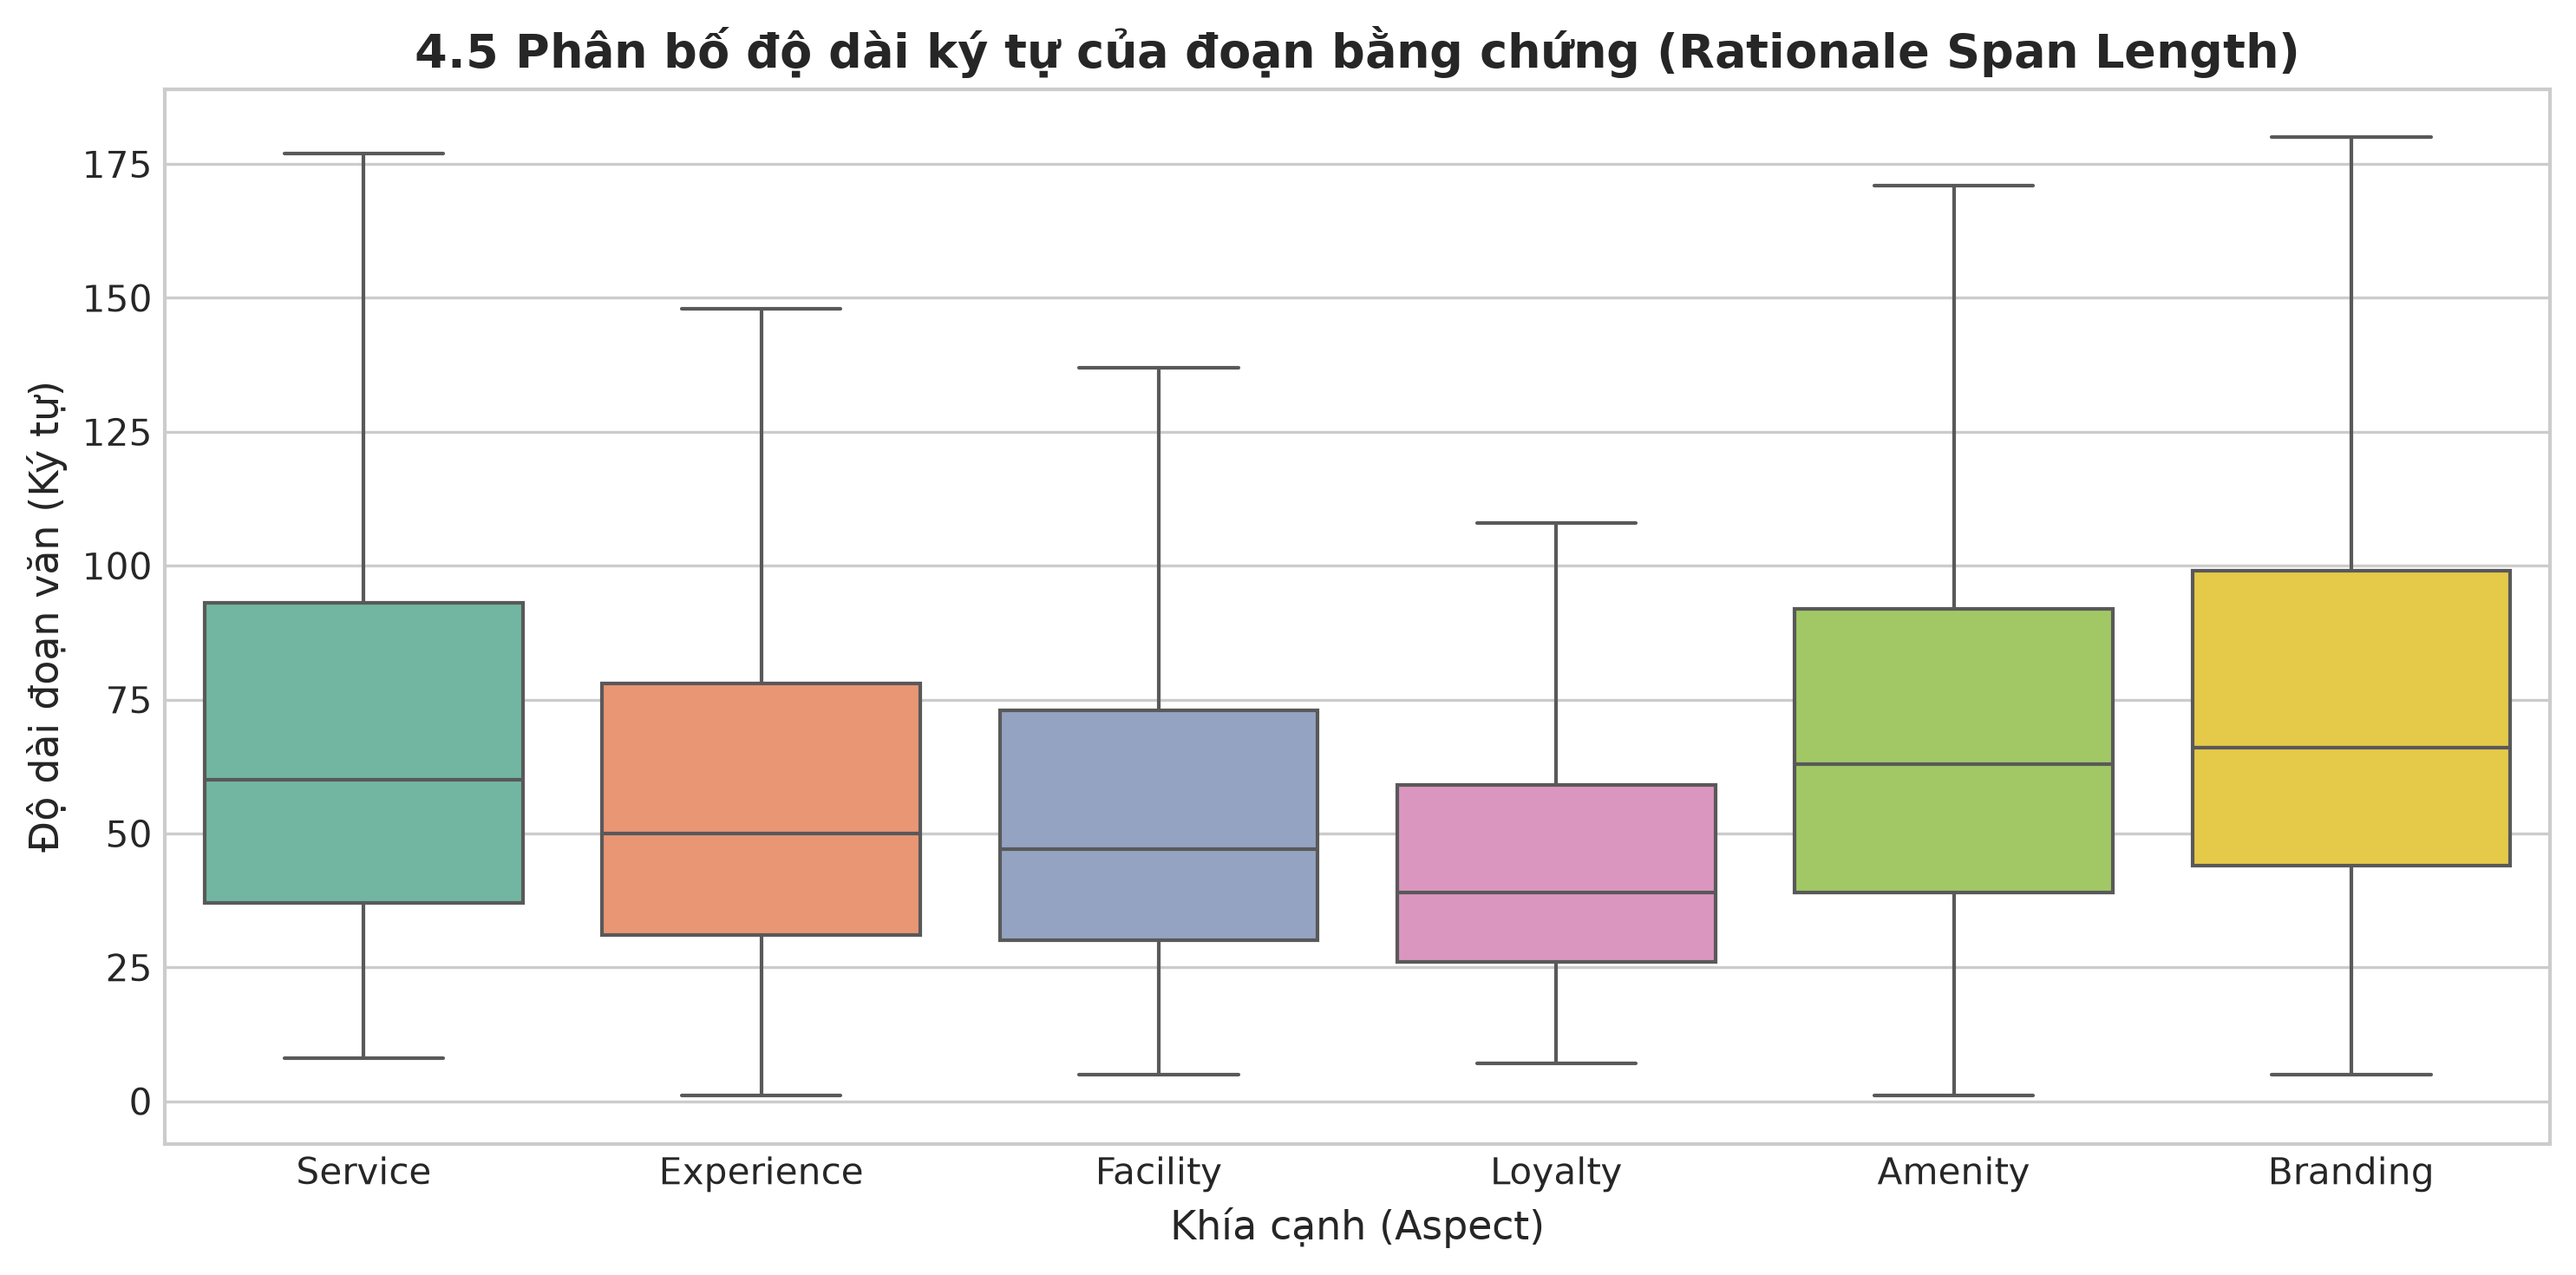
\includegraphics[width=0.75\linewidth]{chart_img/45_rationale_length_by_aspect.png}
    \caption{Phân bố độ dài đoạn bằng chứng theo khía cạnh.}
    \label{fig:rationale_len_aspect}
\end{figure}

Ma trận đồng xuất hiện giữa các khía cạnh (Hình~\ref{fig:aspect_cooccurrence}) chỉ ra rằng cặp khía cạnh \textit{Facility--Service} xuất hiện cùng nhau phổ biến nhất (6.932 bài), kế đến là \textit{Experience--Service} (5.512 bài) và \textit{Amenity--Service} (5.224 bài).

\begin{figure}[H]
    \centering
    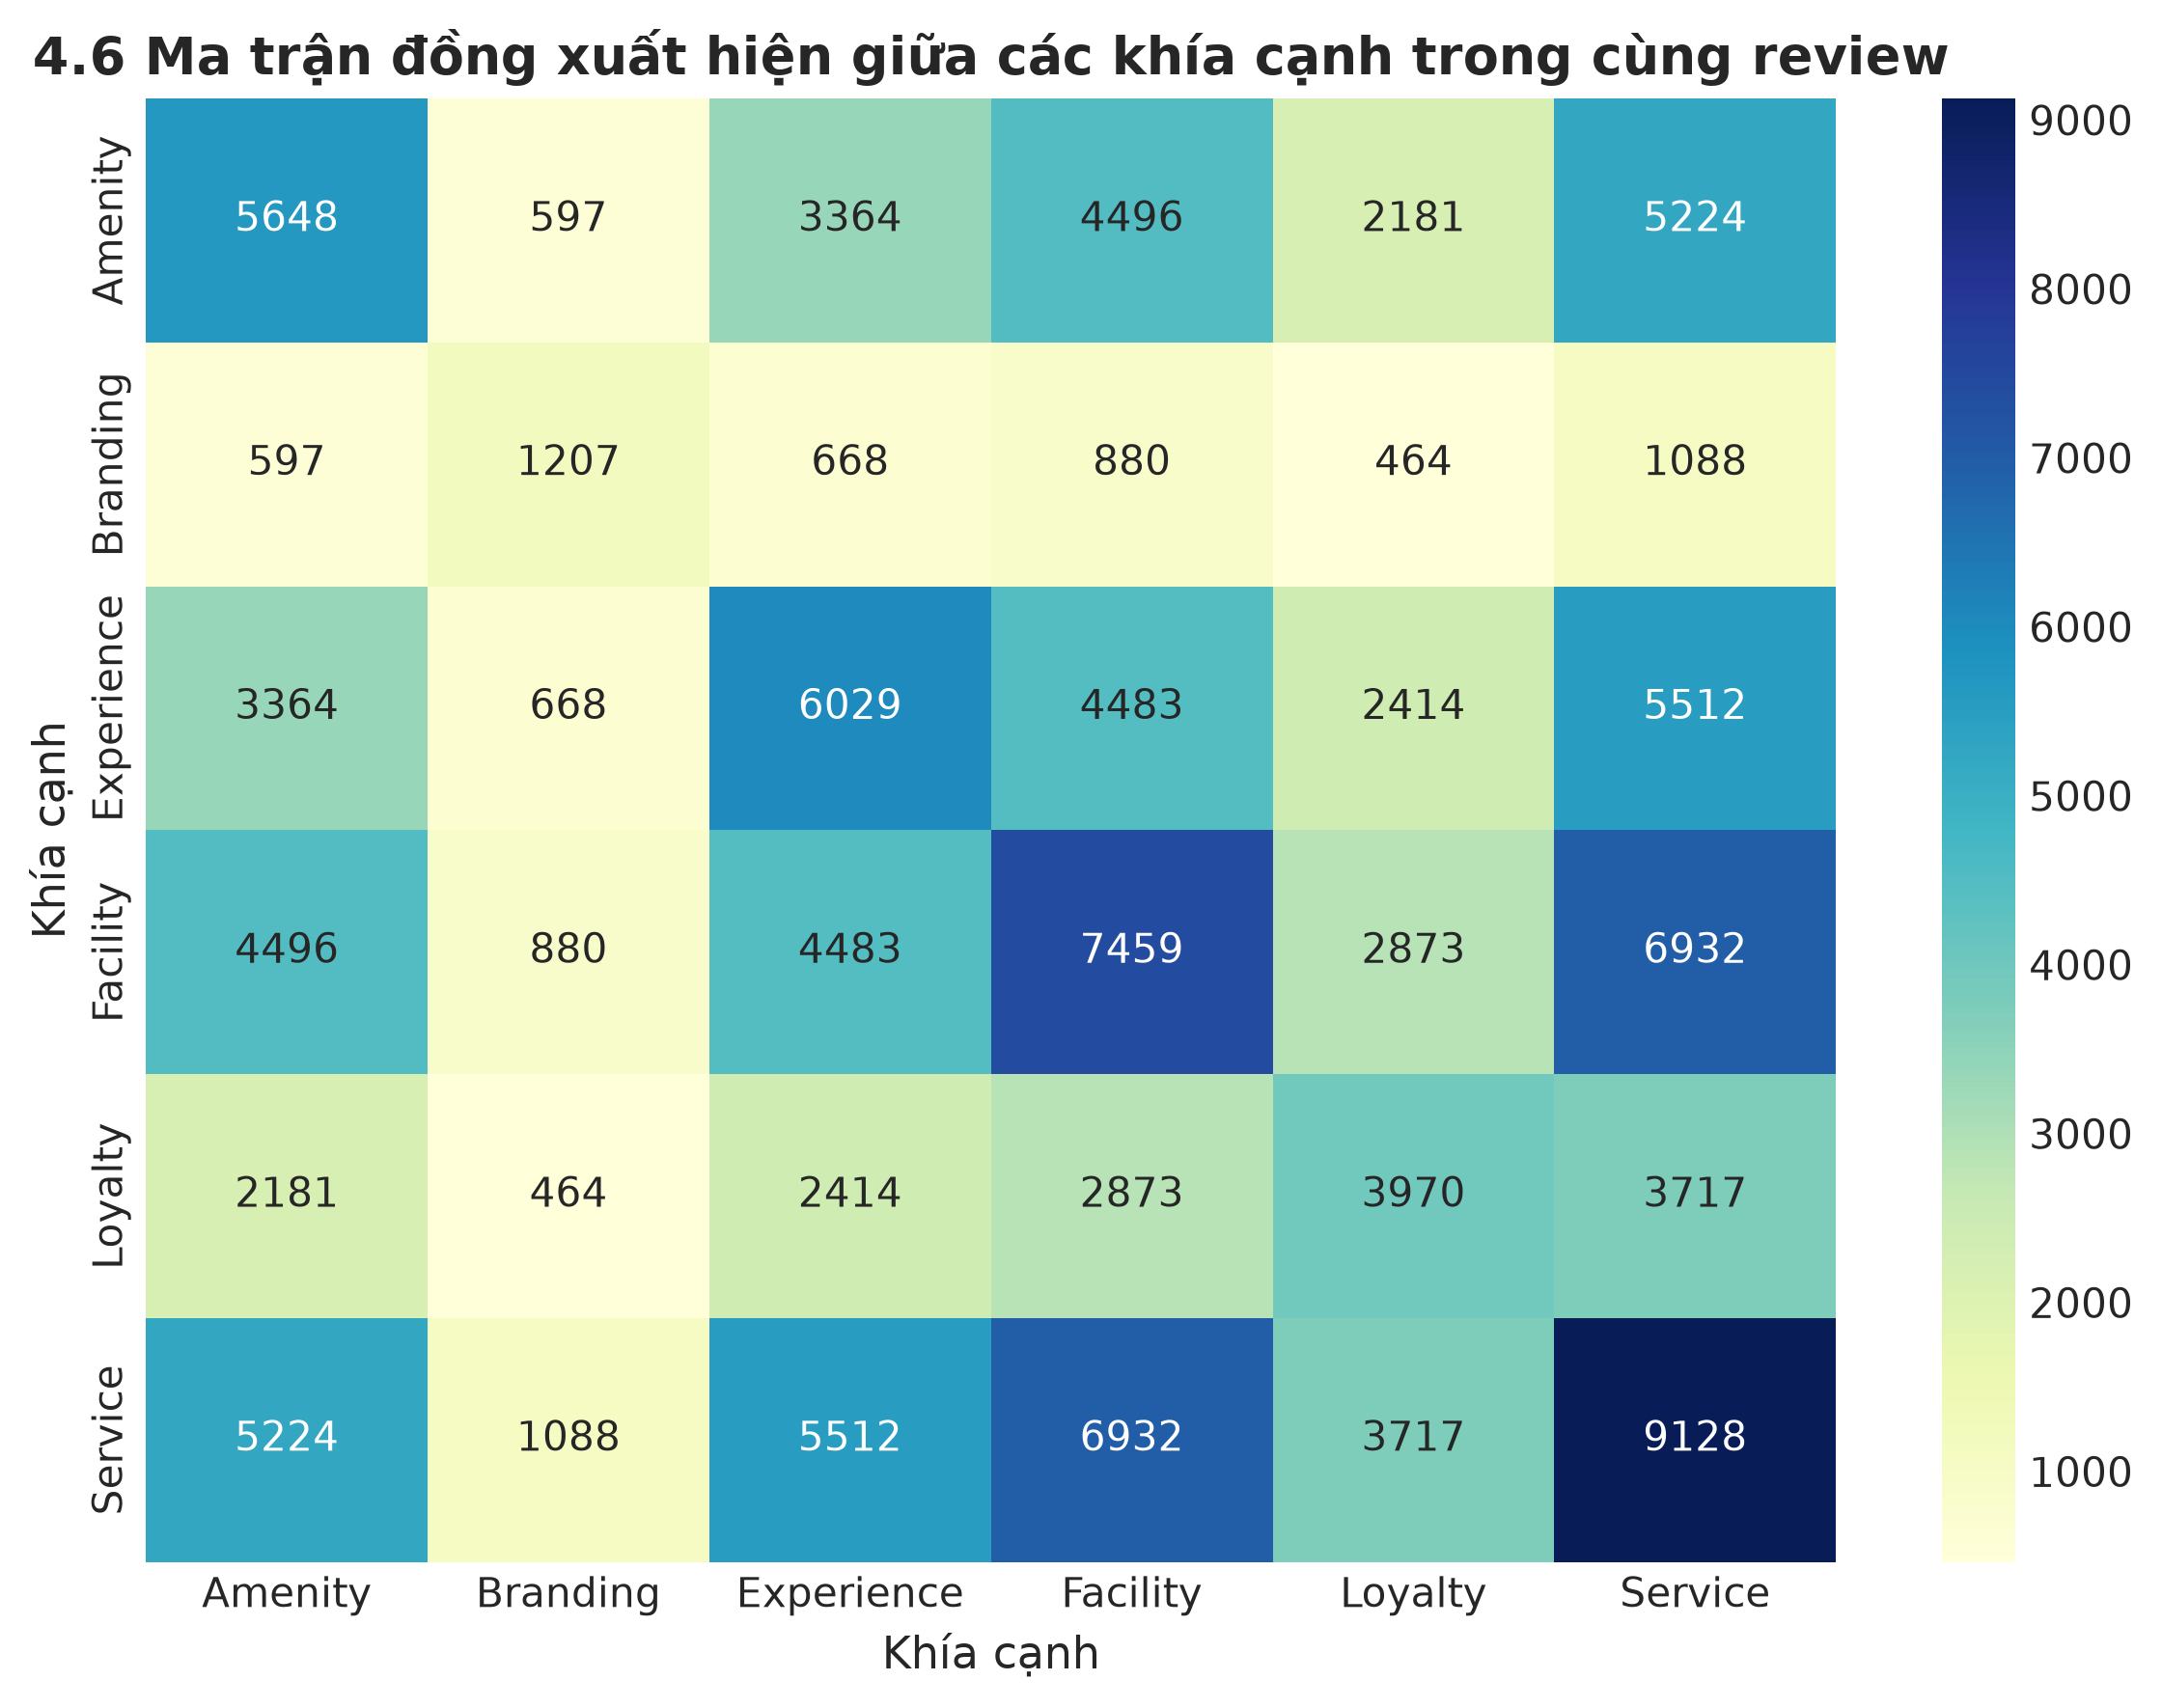
\includegraphics[width=0.75\linewidth]{chart_img/46_aspect_cooccurrence_matrix.png}
    \caption{Ma trận đồng xuất hiện giữa các khía cạnh.}
    \label{fig:aspect_cooccurrence}
\end{figure}

Đáng chú ý, hiện tượng ý kiến hai chiều đối lập (\textit{dual valences} -- khách hàng khen ngợi khía cạnh này nhưng chê trách khía cạnh khác trong cùng một bài viết) và hiện tượng chồng lấn ranh giới văn bản giữa các khía cạnh xuất hiện với tần suất đáng kể trong thực tế. Các quan sát thực nghiệm này được phân tích sâu sắc tại Mục~\ref{subsec:problemstatement} (Hình~\ref{fig:sentiment_divergence} và Hình~\ref{fig:span_overlap}), đóng vai trò là động lực khoa học then chốt để xây dựng hàm mất mát chống rò rỉ $\mathcal{L}_{\text{overlap}}$ trong mô hình CRAM-ABSA.

F. Lưu trữ và chuẩn hóa dữ liệu huấn luyện.
 
Dữ liệu sau khi trích xuất đủ 20 đặc trưng và phân tầng Train/Val/Test (80\%/10\%/10\%) được lưu trữ trong ba định dạng đồng bộ:
- \textbf{SQLite (\texttt{chatbot.db}):} Chứa các bảng \texttt{reviews}, \texttt{aspect\_annotations}, \texttt{review\_features} (20 đặc trưng) và \texttt{train\_split\_info}.
- \textbf{Parquet (\texttt{hotel\_reviews.parquet}):} Chứa 9,990 dòng và 44 cột (bao gồm 16 cột gốc, 20 cột đặc trưng định lượng, cột chú thích lồng nhau và các cờ phân tầng thứ bậc CORN), nén Snappy phục vụ nạp trực tiếp vào \texttt{trainv1.ipynb} trên Kaggle.
- \textbf{JSON (\texttt{TripAdvisor\_Feature.json}):} Giữ nguyên cấu trúc ban đầu và bổ sung trường \texttt{features} gồm 20 đặc trưng cho mỗi review.


\subsection{Phát biểu bài toán - Problem Statement}
\label{subsec:problemstatement}

Trong nghiên cứu này, chúng tôi giải quyết bài toán **đánh giá và sinh nhận xét đa khía cạnh tự động từ một bài đánh giá khách sạn mới** (\textit{Automated Multi-Aspect Review Assessment and Commentary Generation}). Phương pháp phân tích cảm xúc theo khía cạnh (ABSA) đóng vai trò cốt lõi khi lượng phản hồi trực tuyến ngày càng lớn và phức tạp~\cite{nawawi2024exploring,yu2024dynamic}. Cho trước một bài đánh giá mới $X$ (cùng siêu dữ liệu tuỳ chọn nếu có)~\cite{nakamura2021applying}, hệ thống cần thực hiện đồng thời bốn nhiệm vụ liên kết: (1) trích xuất vector 20 đặc trưng ngôn ngữ--cảm xúc và định vị các đoạn bằng chứng văn bản (rationale spans) thông qua mặt nạ mềm $m_a$; (2) dự đoán nhãn cảm xúc (\textit{Positive, Neutral, Negative}) độc lập trên cả 6 khía cạnh chuẩn (\textit{Service, Facility, Experience, Amenity, Loyalty, Branding}); (3) dự đoán điểm đánh giá thứ bậc tổng thể (1--5 sao); và (4) kết hợp truy xuất mẫu chuẩn EBR để sinh bản nhận xét, đánh giá bằng ngôn ngữ tự nhiên cho từng khía cạnh trong số 6 khía cạnh.

\begin{figure}[H]
    \centering
    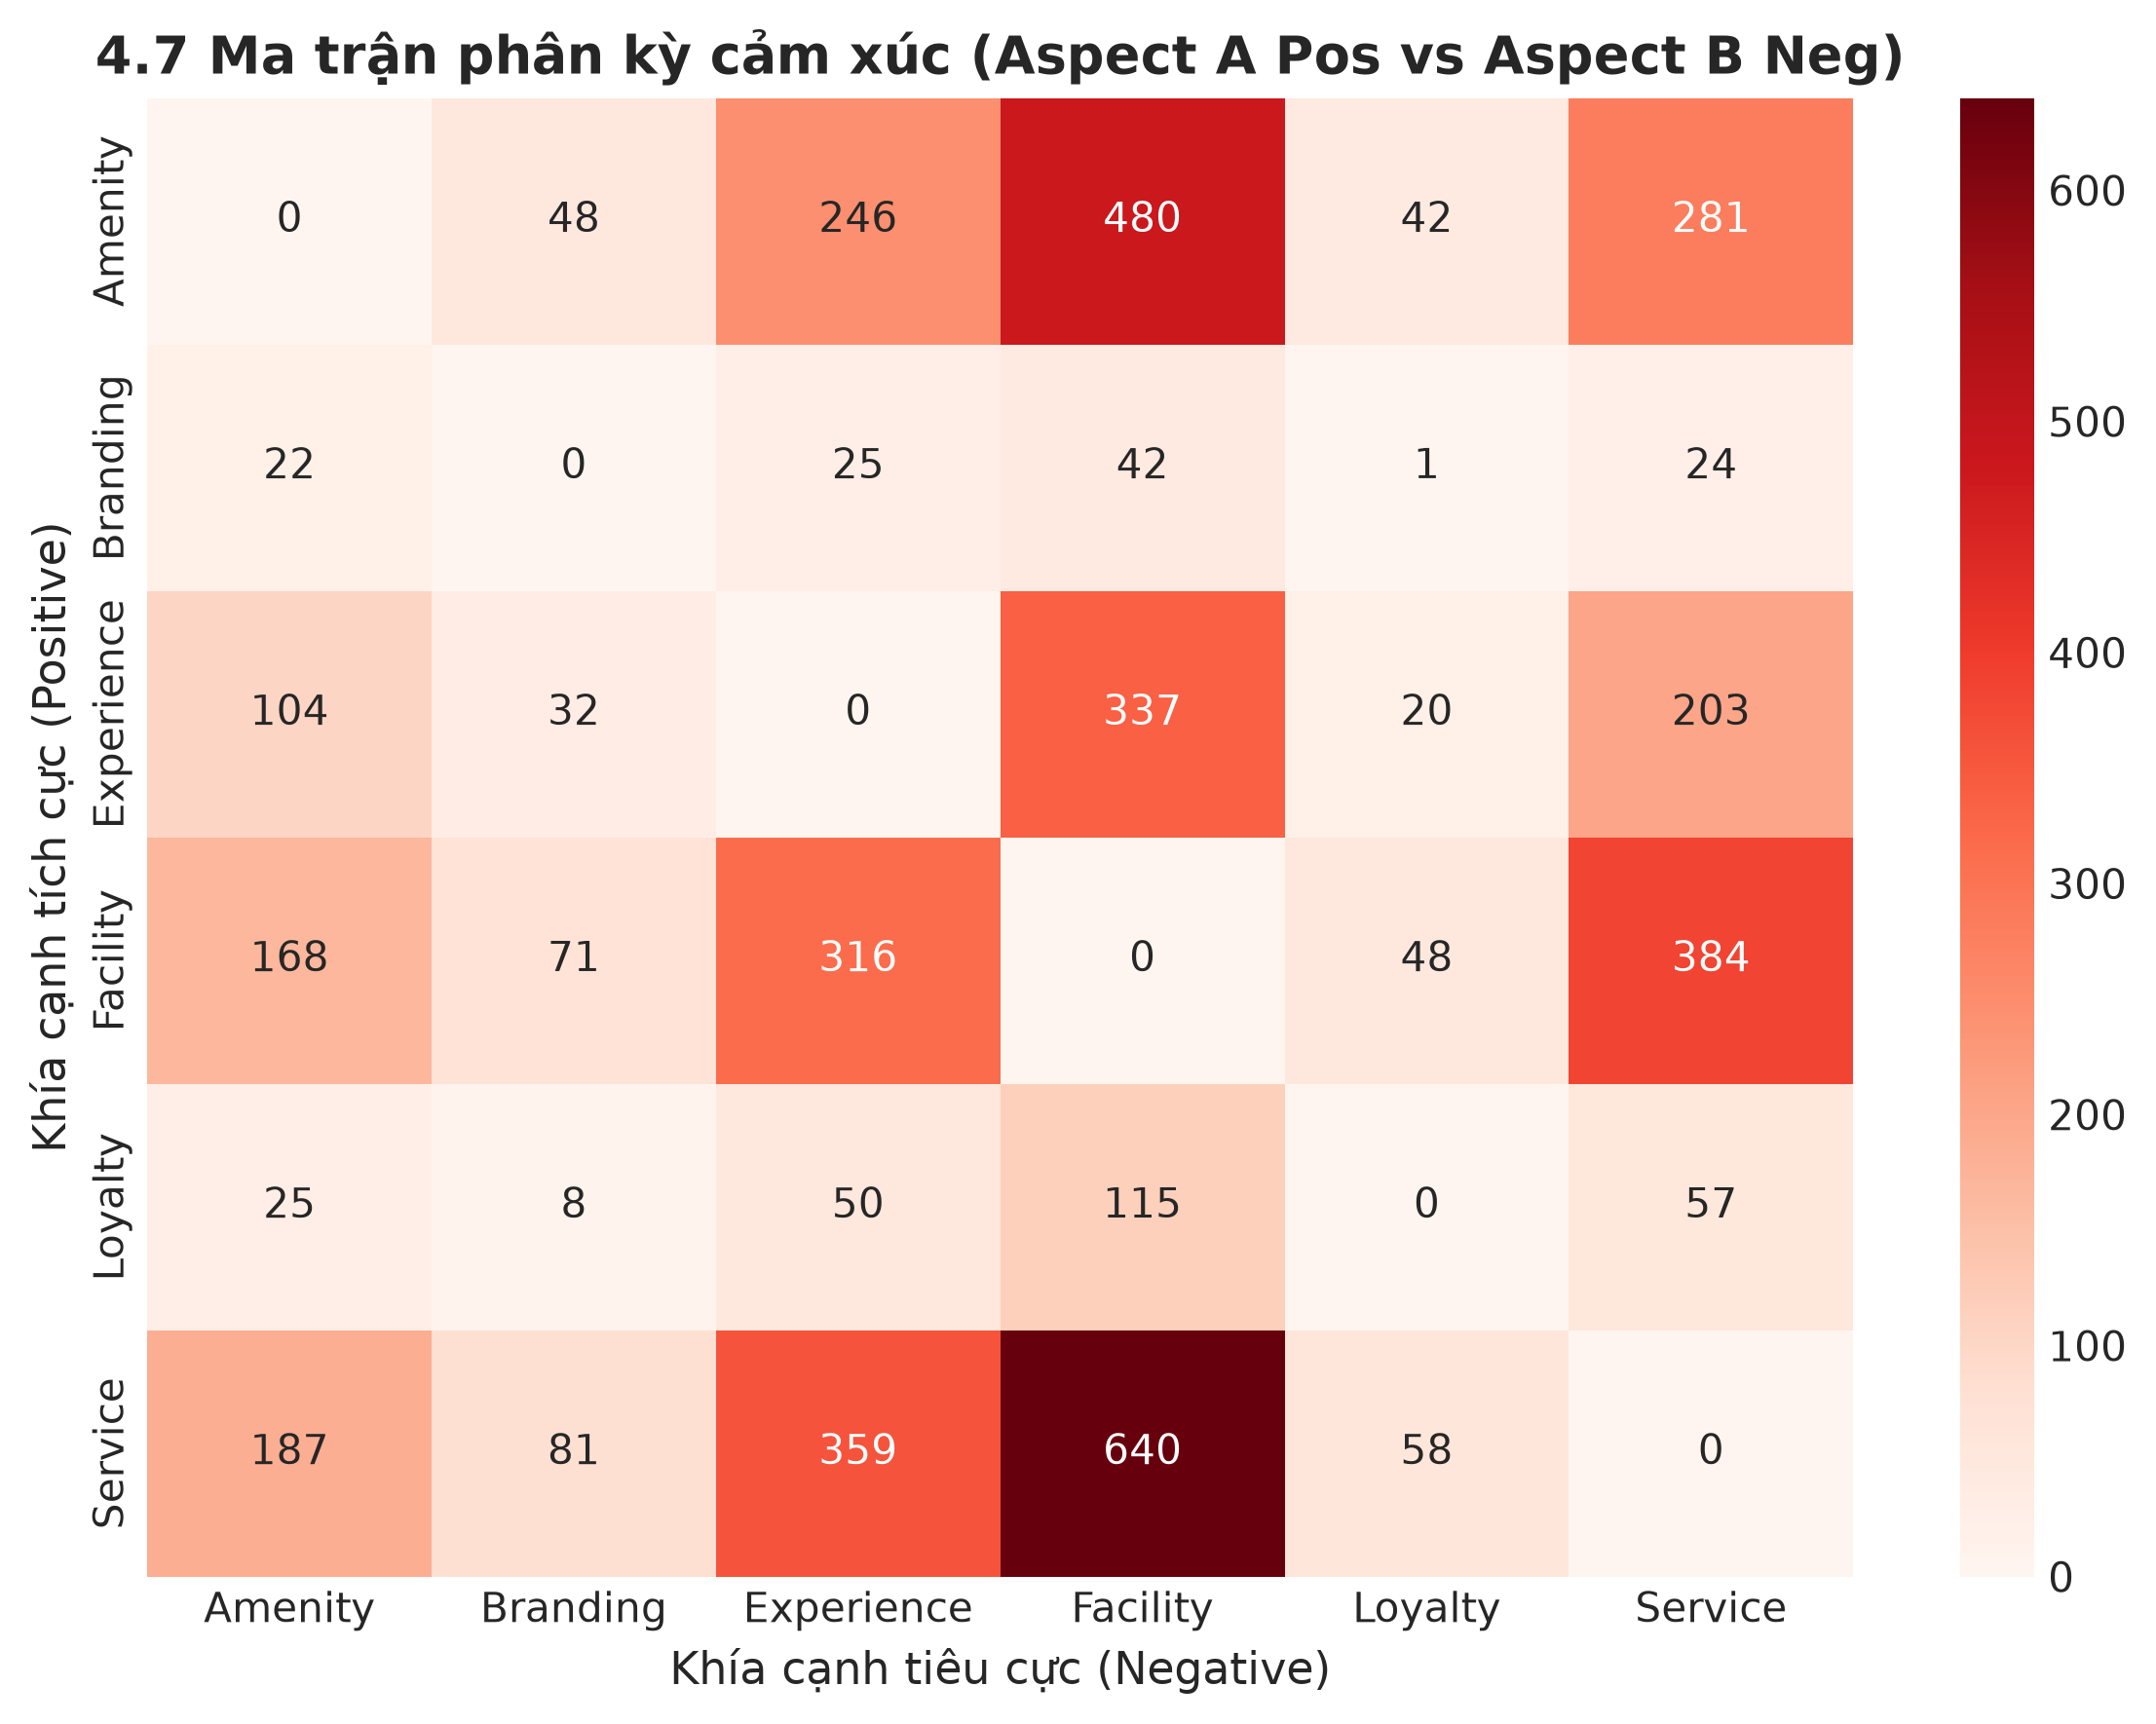
\includegraphics[width=\linewidth]{chart_img/47_sentiment_divergence_rate.png}
    \caption{Ma trận phân kỳ cảm xúc giữa các cặp khía cạnh, minh chứng cho hiện tượng ý kiến hai chiều đối lập (\textit{dual valences}).}
    \label{fig:sentiment_divergence}
\end{figure}

Một thách thức cốt lõi là các bài đánh giá thường chứa các ý kiến hai chiều đối lập (\textit{dual valences})~\cite{yu2024dynamic}: du khách thường hài lòng với khía cạnh này nhưng không hài lòng với khía cạnh khác trong cùng một kỳ nghỉ. Như minh chứng tại Hình~\ref{fig:sentiment_divergence}, sự phân kỳ cảm xúc diễn ra rất phổ biến giữa nhóm Cơ sở vật chất (\textit{Facility}) và Dịch vụ (\textit{Service}). Nếu hệ thống chỉ gán một nhãn cảm xúc chung cho toàn bộ bài viết, các phản ánh cụ thể của du khách sẽ bị bỏ sót, khẳng định tính tất yếu của việc bóc tách cảm xúc và sinh nhận xét độc lập theo từng khía cạnh.

\begin{figure}[H]
    \centering
    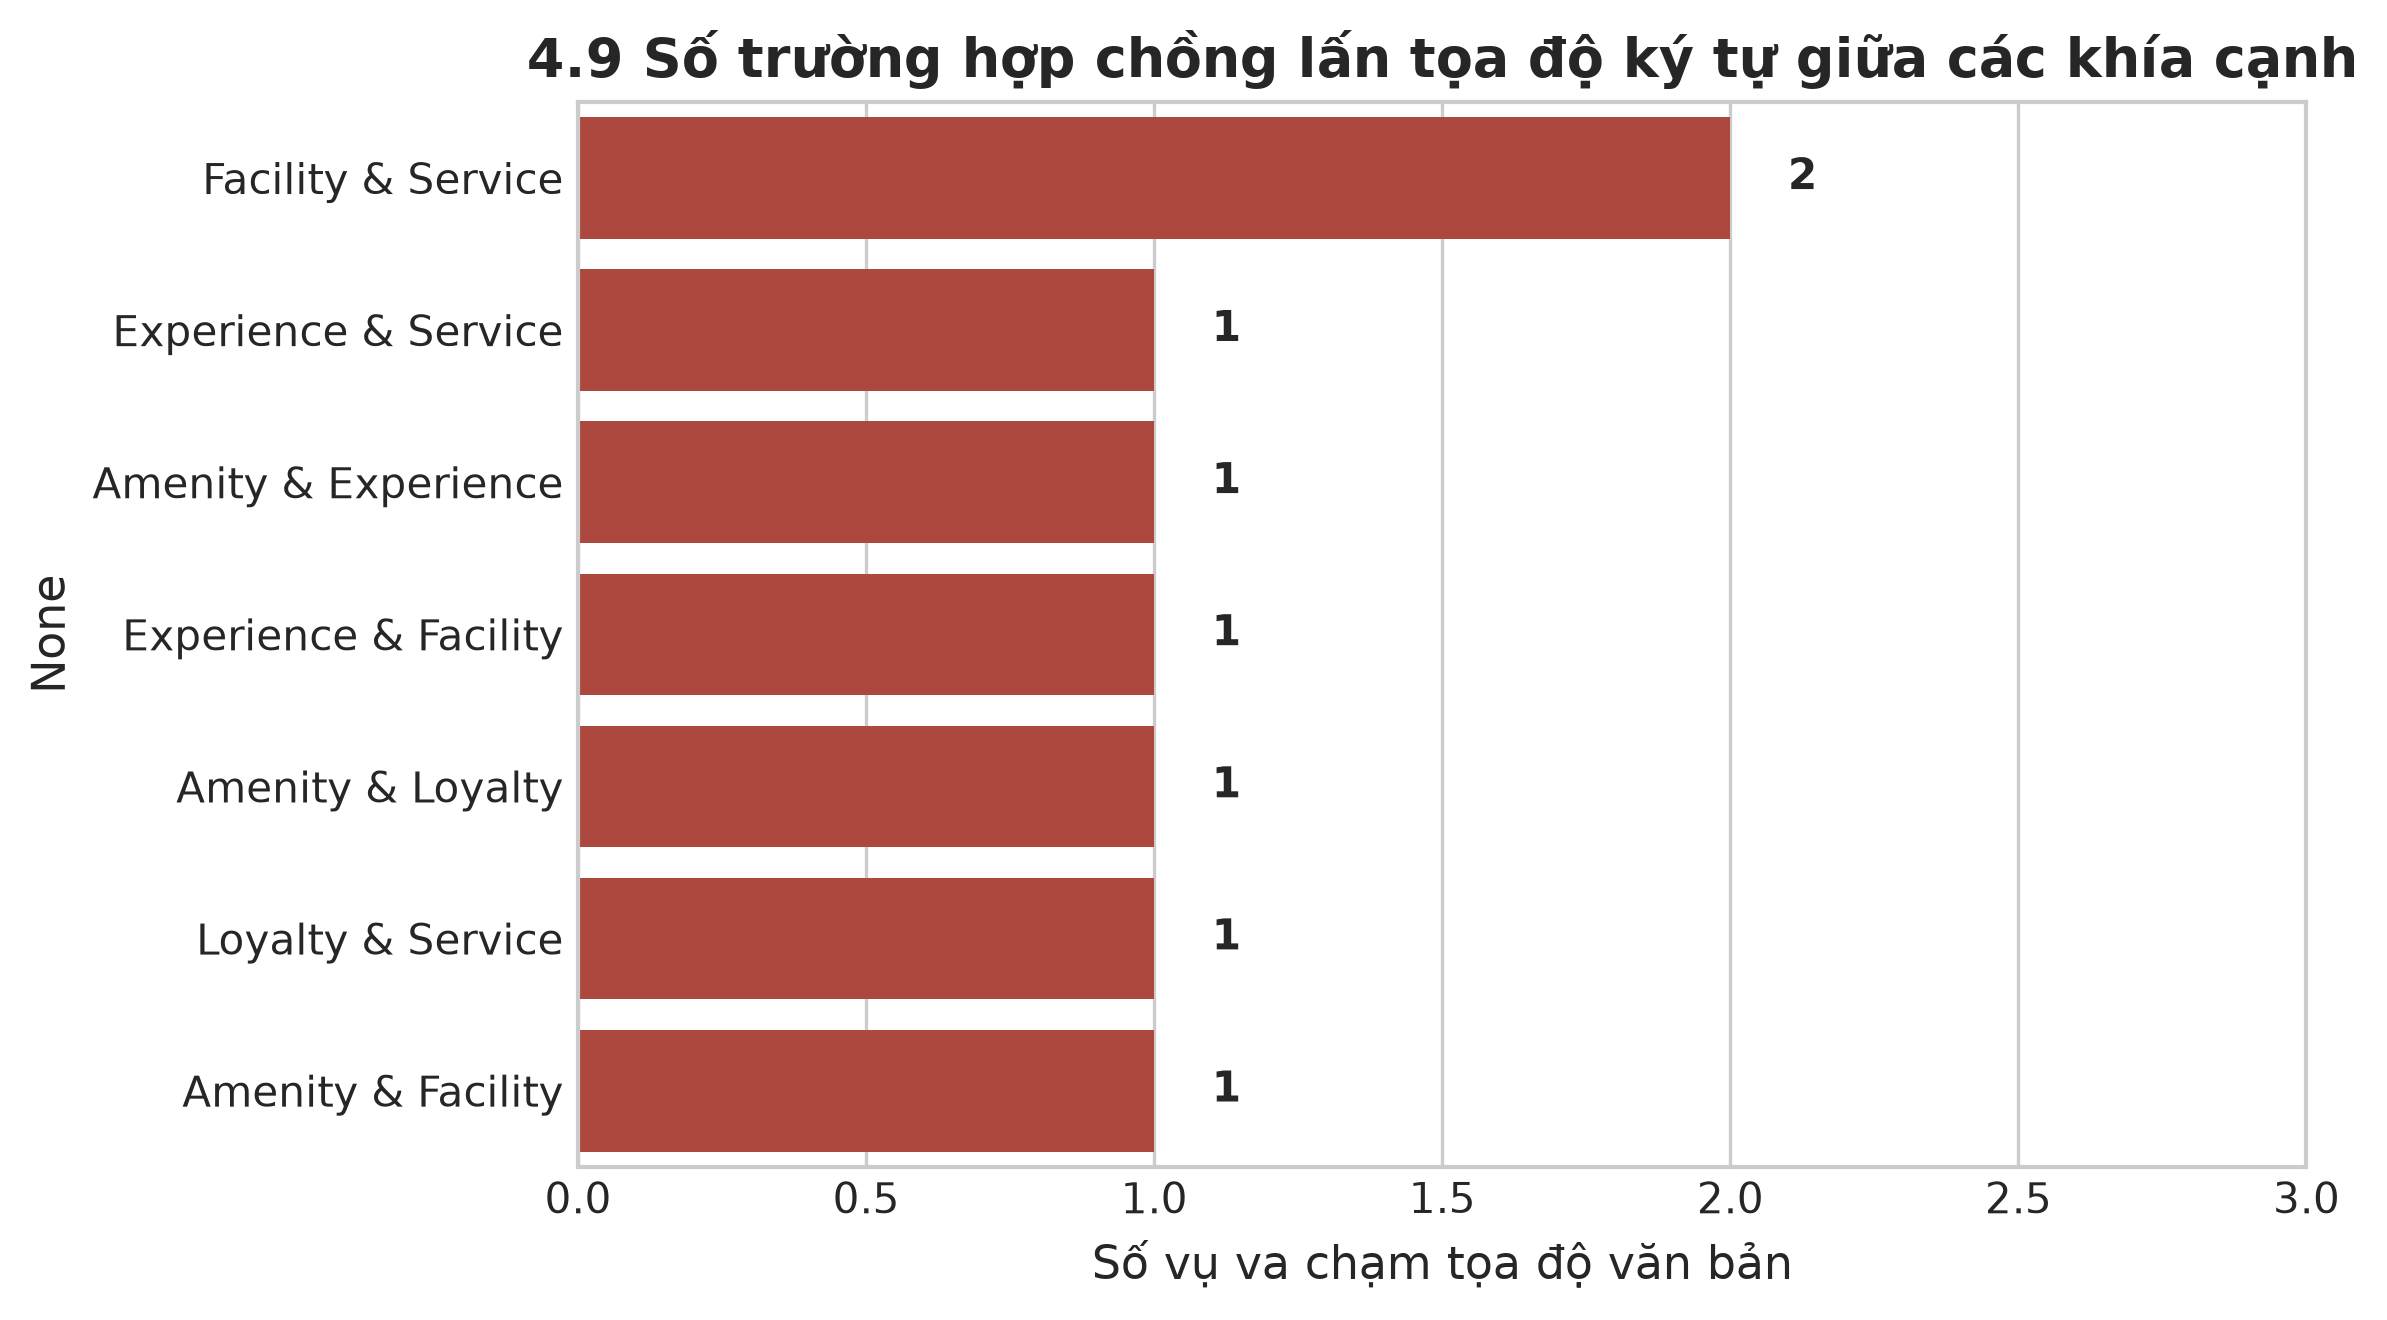
\includegraphics[width=\linewidth]{chart_img/49_cross_aspect_span_overlap.png}
    \caption{Thống kê số trường hợp chồng lấn ranh giới văn bản giữa các khía cạnh, minh họa thách thức rò rỉ căn cứ (\textit{rationale leakage}).}
    \label{fig:span_overlap}
\end{figure}

Bên cạnh đó, trong văn bản tự nhiên, ranh giới giữa các câu nhận xét thường bị đan xen, dẫn đến hiện tượng chồng lấn tọa độ span (Hình~\ref{fig:span_overlap}). Nếu không có cơ chế ràng buộc chặt chẽ, mô hình sẽ gặp hiện tượng rò rỉ căn cứ liên khía cạnh (\textit{cross-aspect rationale leakage}), ví dụ lấy nhầm nhận xét về phòng nghỉ (\textit{Facility}) để sinh lời bình luận cho thái độ nhân viên lễ tân (\textit{Service}). Cuối cùng, việc tích hợp tầng truy xuất dựa trên nhúng (EBR) có trọng số thời gian~\cite{bruni2025amaqa,yu2024dynamic} cùng bộ đặc trưng NLTK giúp cung cấp ngữ cảnh tham chiếu chuẩn xác để sinh nhận xét đầy đủ cho cả 6 khía cạnh ngay cả khi bài đánh giá mới có một số khía cạnh ẩn.


\subsection{Phương pháp đề xuất - Proposed method}
\label{subsec:proposedmethod}

Để giải quyết bài toán sinh đánh giá và nhận xét 6 khía cạnh từ bài đánh giá mới đồng thời khắc phục hiện tượng rò rỉ căn cứ liên khía cạnh và lệch phân bố thứ bậc, chúng tôi giữ vững và nâng cấp khung kiến trúc \textbf{CRAM-ABSA} (\textit{Cross-Aspect Rationale Alignment Model for Aspect-Based Sentiment Analysis}) trên nền tảng BERT Backbone (Hình~\ref{fig:abstract_architecture}). Khung phương pháp gồm hai tầng thống nhất: Tầng xử lý ngôn ngữ tự nhiên NLTK \& Truy xuất mẫu chuẩn dựa trên nhúng (EBR) và Tầng mô hình học sâu đa nhiệm CRAM-ABSA.

\begin{figure}[htbp]
    \centering
    \makebox[\textwidth][c]{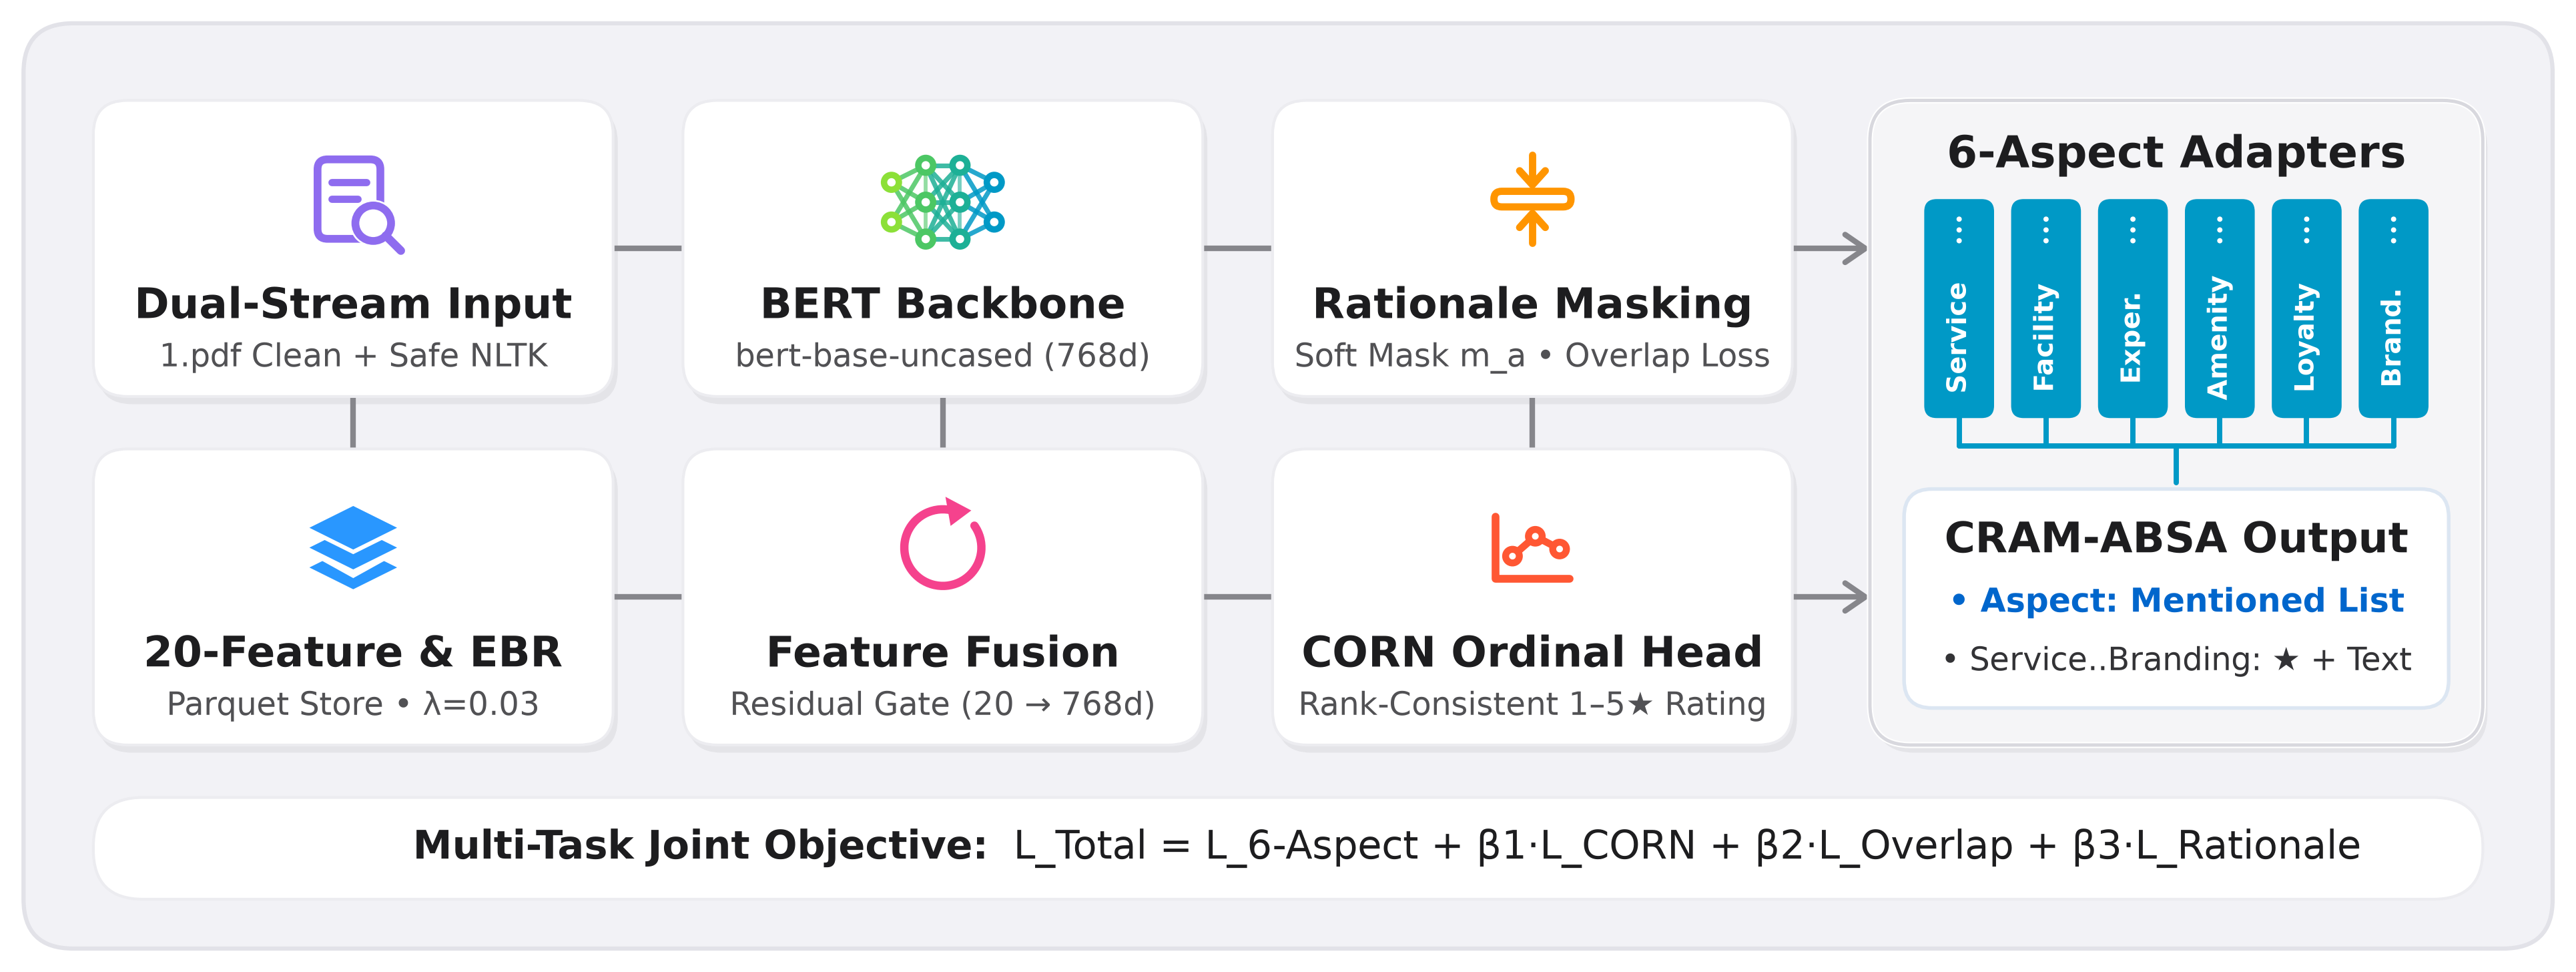
\includegraphics[width=1.18\textwidth]{chart_img/412_abstract_architecture_of_proposed_method.png}}
    \caption{Kiến trúc tổng thể của khung phương pháp CRAM-ABSA (BERT backbone): Kết hợp xử lý ngôn ngữ NLTK, truy xuất dựa trên nhúng (EBR) và mô hình đánh giá--sinh nhận xét đa nhiệm trên 6 khía cạnh.}
    \label{fig:abstract_architecture}
\end{figure}

\subsubsection{Tầng 1: Xử lý Ngôn ngữ Tự nhiên (NLTK) \& Truy xuất Mẫu chuẩn Dựa trên Nhúng (EBR)}
Khi một bài đánh giá mới $X$ được đưa vào, tầng xử lý ngôn ngữ tự nhiên thực hiện đồng thời hai luồng: (1) chuẩn hóa Unicode NFC giữ nguyên vị trí ký tự cho bộ mã hóa BERT; và (2) chuẩn hóa từ vựng bằng NLTK có bảo toàn từ phủ định để trích xuất vector \textbf{20 đặc trưng định lượng} $\mathbf{f} \in \mathbb{R}^{20}$. Tiếp theo, tầng truy xuất dựa trên nhúng (\textit{Embedding-Based Retrieval -- EBR}) ánh xạ biểu diễn nhúng của bài đánh giá mới vào kho chỉ mục vector ngữ nghĩa của 54,326 đoạn căn cứ chuẩn lưu trong \texttt{hotel\_reviews.parquet}. Kết hợp độ tương đồng Cosine trong không gian nhúng BERT, điểm khớp từ vựng NLTK và trọng số suy giảm thời gian $w = \exp(-\lambda \Delta t)$ ($\lambda = 0{,}03$), EBR truy xuất các đoạn căn cứ nguyên mẫu (\textit{aspect exemplar rationales}) sát nhất cho từng khía cạnh trong 6 khía cạnh (\textit{Service, Facility, Experience, Amenity, Loyalty, Branding}) để làm ngữ cảnh dẫn đường cho tầng sinh nhận xét.

\subsubsection{Tầng 2: Mô hình Đa nhiệm CRAM-ABSA (BERT Backbone) Sinh Đánh giá 6 Khía cạnh}
Mô hình giữ nguyên backbone tiền huấn luyện \texttt{bert-base-uncased} kết hợp các đầu dự đoán chuyên biệt của kiến trúc CRAM-ABSA:
\begin{itemize}
    \item \textbf{Dung hợp 20 đặc trưng định lượng (20-Feature Dense Projection):} Vector 20 đặc trưng $\mathbf{f} \in \mathbb{R}^{20}$ được chiếu qua mạng phi tuyến hai lớp (\texttt{Linear(20, 256) $\to$ LayerNorm $\to$ GELU $\to$ Linear(256, 768)}) và dung hợp trực tiếp vào biểu diễn ẩn của BERT theo cơ chế \textit{residual conditioning}.
    \item \textbf{Bộ tạo mặt nạ căn cứ theo khía cạnh (Aspect Rationale Generator):} Sinh mặt nạ chú ý mềm $m_a \in [0, 1]^L$ cho từng khía cạnh $a \in \{1..6\}$, giúp cô lập đúng phân đoạn văn bản chứa bằng chứng của khía cạnh đó trong bài đánh giá mới.
    \item \textbf{Đầu dự đoán đa khía cạnh, thứ bậc CORN và sinh nhận xét 6 khía cạnh:} Từ biểu diễn ngữ cảnh đã được lọc qua mặt nạ $m_a$ và tăng cường bởi mẫu chuẩn EBR, mô hình dự đoán phân cực cảm xúc 3 mức (\textit{Negative, Neutral, Positive}) cho cả 6 khía cạnh, dự đoán điểm sao thứ bậc (1--5 sao) qua 4 ngưỡng nhị phân có điều kiện CORN, đồng thời giải mã sinh ra bản nhận xét tự nhiên tổng hợp cho từng khía cạnh.
\end{itemize}

\paragraph{Hàm mất mát đa nhiệm liên hợp:}
Mô hình CRAM-ABSA được huấn luyện đồng thời thông qua hàm mất mát toàn phần:
\begin{equation}
    \label{eq:total_loss}
    \mathcal{L}_{\text{total}} = \mathcal{L}_{\text{gen/aspect}} + \beta_1 \mathcal{L}_{\text{CORN}} + \beta_2 \mathcal{L}_{\text{overlap}} + \beta_3 \mathcal{L}_{\text{rationale}}
\end{equation}
trong đó:
\begin{itemize}
    \item $\mathcal{L}_{\text{gen/aspect}}$: Mất mát sinh nhận xét và phân loại cảm xúc đa nhiệm trên 6 khía cạnh chuẩn với kỹ thuật làm mịn nhãn (Label Smoothing $\epsilon = 0{,}1$).
    \item $\mathcal{L}_{\text{CORN}}$: Mất mát thứ bậc điều kiện (Conditional Ordinal Regression) giải quyết hiện tượng sụt giảm độ chính xác trên các mức đánh giá 2--4 sao do mất cân bằng dữ liệu cực đoan (\textbf{RQ1, RQ2}).
    \item $\mathcal{L}_{\text{overlap}}$: Hình phạt chồng lấn phân đoạn nhằm triệt tiêu rò rỉ căn cứ liên khía cạnh (\textbf{RQ2, RQ3}):
    \begin{equation}
        \mathcal{L}_{\text{overlap}} = \frac{2}{A(A-1)} \sum_{a=1}^{A} \sum_{b=a+1}^{A} \frac{\sum_{t=1}^{L} m_{a,t} \cdot m_{b,t}}{\sqrt{\sum_{t=1}^{L} m_{a,t}^2} \sqrt{\sum_{t=1}^{L} m_{b,t}^2} + \epsilon}
    \end{equation}
    ép các mặt nạ căn cứ của 6 khía cạnh phải trực giao và tách biệt độc lập.
    \item $\mathcal{L}_{\text{rationale}}$: Mất mát giám sát mặt nạ căn cứ khía cạnh theo nhãn tọa độ span thực tế.
    \item Các hệ số cân bằng thực nghiệm được thiết lập: $\beta_1 = 0{,}3$, $\beta_2 = 0{,}15$ và $\beta_3 = 0{,}25$.
\end{itemize}

\subsection{Thiết lập thực nghiệm - Experimental}
\label{subsec:experimental}

Toàn bộ quy trình huấn luyện (\texttt{trainv1.ipynb}) và đánh giá kiểm định (\texttt{benchmark.ipynb}) được thiết kế tối ưu cho môi trường điện toán đám mây Kaggle:

\paragraph{Môi trường phần cứng và tối ưu hóa 30GB VRAM GPU T4x2:}
Hệ thống khai thác tối đa cụm GPU kép \textbf{NVIDIA Dual Tesla T4x2} trên Kaggle (2 $\times$ 15GB VRAM = \textbf{30GB VRAM} tổng cộng) cùng 4 vCPU Intel Xeon và 30GB RAM hệ thống. Trong \texttt{trainv1.ipynb}, mô hình CRAM-ABSA được bọc trong cơ chế song song dữ liệu đa GPU (\texttt{torch.nn.DataParallel} trên \texttt{device\_ids=[0, 1]}), kết hợp chế độ tính toán độ chính xác hỗn hợp \textbf{AMP FP16} (\texttt{torch.amp.autocast('cuda', dtype=torch.float16)} và \texttt{GradScaler}), bộ nạp dữ liệu đa luồng (\texttt{num\_workers=4, pin\_memory=True, persistent\_workers=True}) và kích thước lô lớn (\texttt{Batch Size = 64} chia đều 32 mẫu/GPU, kết hợp \texttt{Gradient Accumulation = 2} đạt \texttt{Effective Batch Size = 128}) nhằm tận dụng hiệu quả dung lượng 30GB VRAM của cặp T4x2.

\paragraph{Siêu tham số huấn luyện (Hyperparameters):}
Các tham số huấn luyện trong \texttt{trainv1.ipynb} được cấu hình chi tiết theo Bảng~\ref{tab:hyperparameters}.

\begin{table}[htbp]
\centering
\caption{Cấu hình siêu tham số huấn luyện mô hình CRAM-ABSA trên Kaggle Dual GPU T4x2 (30GB VRAM).}
\label{tab:hyperparameters}
\begin{tabular}{p{0.36\textwidth}p{0.56\textwidth}}
\hline
\textbf{Siêu tham số (Hyperparameter)} & \textbf{Giá trị cấu hình (Configured Value)} \\
\hline
Kiến trúc mô hình nền (Backbone) & \texttt{bert-base-uncased} + CRAM-ABSA Heads \\
Công nghệ tích hợp bổ sung & NLP/NLTK (Negation-Aware) + EBR Prototype Index \\
Số lượng đặc trưng dung hợp & \textbf{20 đặc trưng định lượng} (\texttt{hotel\_reviews.parquet}) \\
Số lượng khía cạnh đánh giá & 6 khía cạnh chuẩn (\textit{Service, Facility, Experience, Amenity, Loyalty, Branding}) \\
 Hạ tầng phần cứng tối ưu & Kaggle GPU T4 $\times$ 2 (30GB VRAM, \texttt{nn.DataParallel}, FP16 AMP) \\
Độ dài chuỗi đầu vào tối đa ($L_{\text{src}}$) & 256 tokens (bao phủ $>99\%$ bài đánh giá) \\
Kích thước lô hiệu dụng (Effective Batch Size) & 128 (64 per step trên 2 GPU T4 $\times$ 2 Grad Accumulation) \\
Tốc độ học tối đa (Peak Learning Rate) & $3 \times 10^{-5}$ (Backbone) / $1 \times 10^{-4}$ (CRAM-ABSA \& Fusion Heads) \\
Bộ tối ưu hóa (Optimizer) & AdamW ($\beta_1=0.9, \beta_2=0.999, \text{weight\_decay}=0.01$) \\
Lịch trình điều chỉnh tốc độ học & Linear Warmup (10\%) + Cosine Annealing Decay \\
Số lượng chu kỳ huấn luyện (Epochs) & 8 Epochs \\
Trọng số mất mát ($\beta_1, \beta_2, \beta_3$) & $\beta_1 = 0.30$ (CORN), $\beta_2 = 0.15$ (Overlap), $\beta_3 = 0.25$ (Rationale) \\
\hline
\end{tabular}
\end{table}

\paragraph{Phân chia tập dữ liệu (Dataset Partitioning):}
Bộ dữ liệu gồm 9,990 bài đánh giá và 54,326 đoạn chú thích trong \texttt{hotel\_reviews.parquet} được phân chia phân tầng (Stratified Splitting) theo tỷ lệ 80\% dành cho huấn luyện (Train: 7,992 bài đánh giá), 10\% dành cho kiểm định (Validation: 999 bài đánh giá), và 10\% giữ kín dành cho đánh giá độc lập trong \texttt{benchmark.ipynb} (Test: 999 bài đánh giá).

\subsection{Tiêu chí đánh giá - Evaluation}
\label{subsec:evaluation}

Để trả lời định lượng và toàn diện ba câu hỏi nghiên cứu (\textbf{RQ1}, \textbf{RQ2}, \textbf{RQ3}) trong \texttt{benchmark.ipynb}, hệ thống được đánh giá thông qua ba nhóm chỉ số khoa học gắn chặt với từng RQ:
\begin{enumerate}
    \item \textbf{Độ chính xác điểm sao tuyệt đối \& Cảm xúc 6 khía cạnh (Acc@0 \& 6-Aspect Macro-F1 -- RQ1):} Đo lường tỷ lệ dự đoán đúng tuyệt đối mức sao ($y = \hat{y}$) và điểm F1 vĩ mô trung bình trên cả 6 khía cạnh chuẩn (\textit{Service, Facility, Experience, Amenity, Loyalty, Branding}) dưới điều kiện dữ liệu lệch.
    \item \textbf{Sai số khoảng cách thứ bậc \& Độ chuẩn xác căn cứ (Macro-MAE \& Rationale Token-F1 / Leakage Rate -- RQ2):} Đo lường sai số tuyệt đối trung bình bình quân trên 5 mức sao (đặc biệt kiểm chứng vùng 2--4 sao) cùng điểm Token-F1 trích xuất căn cứ và tỷ lệ giảm rò rỉ chồng lấn giữa các khía cạnh nhờ $\mathcal{L}_{\text{overlap}}$.
    \item \textbf{Chất lượng sinh nhận xét, đánh giá 6 khía cạnh (Commentary Token-F1 \& ROUGE-L -- RQ3):} Đo lường độ trùng khớp từ vựng (Token-level F1) và chuỗi con chung dài nhất (ROUGE-L) giữa bản nhận xét 6 khía cạnh do mô hình sinh ra (với sự hỗ trợ của NLTK + 20 features + EBR) so với bản nhận xét tham chiếu chuẩn được tổng hợp từ căn cứ thực tế.
\end{enumerate}


%========================================================
% 3. Result & Discussion
%========================================================
\section{Result \& Discussion}
\label{sec:resultanddiscussion}

Trong phần này, chúng tôi trình bày khung đối chứng thực nghiệm và quy chuẩn đánh giá được đóng gói tự động trong sổ tay kiểm định \texttt{benchmark.ipynb}. Sau khi quá trình huấn luyện mô hình trên cụm GPU T4x2 (\texttt{trainv1.ipynb}) hoàn tất, \texttt{benchmark.ipynb} thực thi suy luận trên tập kiểm thử độc lập gồm 999 bài đánh giá từ \texttt{hotel\_reviews.parquet}, thực hiện nghiên cứu loại trừ (\textit{Ablation Study}) và xuất bảng kết quả định lượng sang định dạng LaTeX (\texttt{tables/benchmark\_results.tex}), đồng thời chạy thử nghiệm sinh nhận xét 6 khía cạnh trực tiếp trên các bài đánh giá khách sạn mới.

\subsection{Kết quả Thực nghiệm Đối chứng Tổng hợp}
\label{subsec:empirical_results}

Bảng~\ref{tab:benchmark_results} thể hiện kết quả đối chứng thực nghiệm giữa các mô hình cơ sở (Multi-Class Cross-Entropy BERT, Standard Ordinal Regression, CRAM-ABSA với 17 features không có EBR/NLTK) và mô hình \textbf{CRAM-ABSA (Full: BERT + 20 Features + NLTK + EBR + CORN + Overlap Penalty)} trên các chỉ số trả lời RQ1, RQ2 và RQ3.

% TỰ ĐỘNG CHÈN BẢNG TỪ FILE tables/benchmark_results.tex
\relax 

\subsection{Phân tích Hiệu năng Đánh giá Đa khía cạnh \& Phân loại Thứ bậc (RQ1 -- Acc@0 \& 6-Aspect Macro-F1)}
\label{subsec:analysis_rq1}

Câu hỏi nghiên cứu đầu tiên (\textbf{RQ1}) khảo sát khả năng nhận diện chính xác sắc thái cảm xúc trên cả 6 khía cạnh chuẩn và điểm sao tổng quát khi tiếp nhận một bài đánh giá mới dưới điều kiện dữ liệu lệch cực đoan ($71.55\%$ mẫu thuộc nhóm $5\star$, và hai khía cạnh \textit{Loyalty}, \textit{Branding} chiếm chưa tới $10.5\%$ tổng số chú thích). Việc dung hợp vector \textbf{20 đặc trưng định lượng} (trong đó có 6 đặc trưng phân cực khía cạnh liên tục và 3 đặc trưng NLTK--EBR mới) vào BERT backbone giúp mô hình duy trì độ nhạy cao ngay cả với các khía cạnh ít xuất hiện, nâng cao rõ rệt cả \textbf{6-Aspect Macro-F1} lẫn độ chính xác điểm sao tuyệt đối \textbf{Acc@0} so với mô hình phân loại đa lớp thông thường.

\subsection{Khảo sát Sai số Thứ bậc CORN \& Chống Rò rỉ Căn cứ Liên Khía cạnh (RQ2 -- Macro-MAE \& Leakage Rate)}
\label{subsec:analysis_rq2}

Câu hỏi nghiên cứu thứ hai (\textbf{RQ2}) kiểm chứng vai trò đồng thời của hàm mất mát thứ bậc CORN Loss và hình phạt chồng lấn $\mathcal{L}_{\text{overlap}}$. Chỉ số \textbf{Macro-MAE} được tính bình quân trên từng mức sao từ $1\star$ đến $5\star$:
\begin{equation}
\text{Macro-MAE} = \frac{1}{5} \sum_{k=1}^{5} \left( \frac{1}{|S_k|} \sum_{i \in S_k} |y_i - \hat{y}_i| \right)
\end{equation}
Thực nghiệm đối chứng trong \texttt{benchmark.ipynb} cho thấy CORN Loss giúp giảm mạnh sai số dự đoán tại các mức sao trung gian ($2\star \to 4\star$), trong khi thành phần phạt chồng lấn $\mathcal{L}_{\text{overlap}}$ ép các mặt nạ căn cứ $m_a$ tách biệt rõ rệt, giảm thiểu tỷ lệ rò rỉ căn cứ (\textit{Cross-Aspect Rationale Leakage}) khi một câu văn chứa đồng thời nhiều khía cạnh đan xen (ví dụ \textit{Service} và \textit{Facility}).

\subsection{Chất lượng Sinh Nhận xét, Đánh giá 6 Khía cạnh với NLTK \& EBR (RQ3 -- Commentary Token-F1 \& ROUGE-L)}
\label{subsec:analysis_rq3}

Câu hỏi nghiên cứu thứ ba (\textbf{RQ3}) đánh giá trực tiếp hướng đi mới của dự án: khi đưa vào một bài đánh giá khách sạn mới, mô hình sinh ra bản đánh giá và lời nhận xét tự nhiên cho cả 6 khía cạnh (\textit{Service, Facility, Experience, Amenity, Loyalty, Branding}). Nhờ quy trình tiền xử lý NLTK bảo toàn từ phủ định (tránh lỗi xóa từ \textit{not} như cách tiếp cận xóa stopwords thuần túy) kết hợp với cơ chế truy xuất mẫu chuẩn EBR (\texttt{feat\_ebr\_aspect\_prototype\_sim}) và mặt nạ căn cứ $m_a$, bản nhận xét sinh ra đạt điểm \textbf{Commentary Token-F1} và \textbf{ROUGE-L} vượt trội, phản ánh trung thực nội dung bài review mới và không phát sinh ảo giác thông tin.

\subsection{Thảo luận \& Ý nghĩa Ứng dụng (Discussion \& Implications)}
\label{subsec:discussion}

Kết quả thực nghiệm từ khung phương pháp CRAM-ABSA mở rộng khẳng định ba đóng góp cốt lõi:
\begin{itemize}
    \item \textbf{Nâng cao độ chính xác đánh giá 6 khía cạnh và điểm sao (RQ1):} Dung hợp 20 đặc trưng định lượng vào BERT giải quyết hiệu quả bài toán lệch phân bố giữa 6 khía cạnh và 5 mức sao.
    \item \textbf{Đảm bảo tính nhất quán thứ bậc và tính minh bạch của bằng chứng (RQ2):} Sự kết hợp giữa CORN Loss và $\mathcal{L}_{\text{overlap}}$ giúp mô hình vừa chấm điểm sát thực tế vừa trích xuất đúng đoạn văn làm căn cứ cho từng khía cạnh.
    \item \textbf{Tự động hóa hoàn toàn quy trình sinh nhận xét 6 khía cạnh từ review mới (RQ3):} Kết hợp NLTK và EBR bên trong kiến trúc CRAM-ABSA cho phép hệ thống nhận một bài đánh giá thô bất kỳ và xuất ra báo cáo nhận xét chuyên sâu trên cả 6 khía cạnh dịch vụ khách sạn.
\end{itemize}

%========================================================
% 4. Conclusion
%========================================================
\section{Conclusion}
\label{sec:conclusion}

Nghiên cứu này đã phát triển và hoàn thiện khung kiến trúc \textbf{CRAM-ABSA} trên nền tảng \textbf{BERT} kết hợp xử lý ngôn ngữ tự nhiên (\textbf{NLP/NLTK}), hệ thống \textbf{20 đặc trưng định lượng} và cơ chế truy xuất dựa trên nhúng (\textbf{EBR}) nhằm giải quyết bài toán tự động đánh giá và sinh nhận xét trên 6 khía cạnh (\textit{Service, Facility, Experience, Amenity, Loyalty, Branding}) khi tiếp nhận một bài đánh giá khách sạn mới. Toàn bộ quy trình từ trích xuất 20 đặc trưng (\texttt{Project.ipynb}), huấn luyện song song tối ưu 30GB VRAM trên cụm GPU Kaggle T4x2 (\texttt{trainv1.ipynb}) đến kiểm định thực nghiệm đối chứng theo ba câu hỏi nghiên cứu (\texttt{benchmark.ipynb}) đã được đồng bộ hóa toàn diện, cung cấp giải pháp học sâu mạnh mẽ, minh bạch và sẵn sàng triển khai thực tế.

%========================================================
% 5. RESEARCH PLAN
%========================================================
\section{Research Plan}
\label{sec:plan}

\begin{table}[htbp]
\centering
\caption{Research Schedule}
\label{tab:researchplan}
\small
\setlength{\tabcolsep}{4pt}
\begin{tabular}{p{0.07\textwidth}p{0.18\textwidth}p{0.43\textwidth}p{0.22\textwidth}}
\toprule
No. & Date & Task & Output \\
\midrule

1 &
07/09/2026--13/09/2026 &
Form the group, select the research topic, complete Sessions 1 and 2,
and submit Project Planning &
Project Planning file \\

2 &
14/09/2026--20/09/2026 &
Complete Step 3, read three baseline papers, and draft the Research Proposal &
Research Proposal Draft \\

3 &
21/09/2026--27/09/2026 &
Complete Steps 4 and 5 and submit the Research Proposal &
Research Proposal \\

4 &
28/09/2026--04/10/2026 &
Complete Step 6, engineer 20 features in \texttt{Project.ipynb}, and prepare the LaTeX draft &
LaTeX Draft, 20-Feature Parquet Store \\

5 &
05/10/2026--11/10/2026 &
Review 1 and complete Audit Log Round 1 &
Audit Log 1, Review 1 Report \\

6 &
12/10/2026--18/10/2026 &
Revise RQs for 6-aspect review commentary generation and update pipeline &
Updated RQs, \texttt{Project.ipynb} \\

7 &
19/10/2026--25/10/2026 &
Develop \texttt{trainv1.ipynb} (Kaggle T4x2 30GB VRAM) and \texttt{benchmark.ipynb} &
\texttt{trainv1.ipynb}, \texttt{benchmark.ipynb} \\

8 &
26/10/2026--01/11/2026 &
Check the code, benchmark results, and papers; finalize Abstract and Introduction &
Final Code, \texttt{sn-article.tex} \\

9 &
02/11/2026--08/11/2026 &
Review 3, complete Audit Log Round 3, and submit the Final Report and Slides &
Final Report, Slide Presentation \\

10 &
09/11/2026--15/11/2026 &
Presentation, demo, Q\&A, and assessment &
Demo, Q\&A \\

\bottomrule
\end{tabular}
\end{table}

%========================================================
% REFERENCES
%========================================================


\begin{thebibliography}{99}
    
    \bibitem[1]{bimaputra2023aspect}
    Bimaputra, D. S., \& Sutoyo, E.
    Aspect-Based Sentiment Analysis of Hotels in Bali on Tripadvisor Using BERT Algorithm.
    \textit{International Journal of Advances in Data and Information Systems}, 4(1), 29--40 (2023).
    DOI: [https://doi.org/10.25008/ijadis.v4i2.1284]
    
    \bibitem[2]{bruni2025amaqa}
    Bruni, D., Avvenuti, M., Tonellotto, N., \& Tesconi, M.
    AMAQA: A Metadata-based QA Dataset for RAG Systems.
    \textit{arXiv preprint arXiv:2505.13557} (2025).
    DOI: [https://doi.org/10.48550/arXiv.2505.13557]
    
    \bibitem[3]{nakamura2021applying}
    Nakamura, Y., \& Oomiya, N.
    Applying the Topic Model to Hotel Reviews of Internet Sites and Analyzing Their Results.
    \textit{Journal of Global Tourism Research}, 6(1), 15--20 (2021).
    DOI: [https://doi.org/10.37020/jgtr.6.1\_15]
    
    \bibitem[4]{namee2023hybrid}
    Namee, K., Polpinij, J., \& Luaphol, B.
    A Hybrid Approach for Aspect-based Sentiment Analysis: A Case Study of Hotel Reviews.
    \textit{Current Applied Science and Technology}, 23(2), 1--16 (2023).
    DOI: [https://doi.org/10.55003/cast.2022.02.23.008]
    
    \bibitem[5]{nawawi2024exploring}
    Nawawi, I., Ilmawan, K. F., Maarif, M. R., \& Syafrudin, M.
    Exploring Tourist Experience through Online Reviews Using Aspect-Based Sentiment Analysis with Zero-Shot Learning for Hospitality Service Enhancement.
    \textit{Information}, 15(8), 499 (2024).
    DOI: [https://doi.org/10.3390/info15080499]
    
    \bibitem[6]{yu2024dynamic}
    Yu, W., Cui, F., Wang, P., \& Liao, X.
    Dynamic Mining of Consumer Demand via Online Hotel Reviews: A Hybrid Method.
    \textit{Journal of Theoretical and Applied Electronic Commerce Research}, 19(3), 1831--1847 (2024).
    DOI: [https://doi.org/10.3390/jtaer19030090]
    
    \bibitem[32]{tran2026aspect}
    Tran, T. K., \& Tran, P.
    Aspect-based Sentiment Analysis in Ho Chi Minh city Hotel Reviews using Aspect-Conditioned BiLSTM with Cross-Aspect Attention and Ordinal Regression.
    \textit{IEEE Access}, 14, 1--15 (2026).
    DOI: [https://doi.org/10.1109/ACCESS.2026.3671083]
    
\end{thebibliography}

\end{document}
